\documentclass[11pt,a4paper,oneside]{report}

\usepackage[T1]{fontenc}
\usepackage[utf8]{inputenc}
\usepackage[romanian]{babel}
% Narrow margins on purpose. The figures are screenshots of a 1440-pixel-wide
% screen, so every centimetre of text width is a centimetre of legibility for
% the formulas inside them.
\usepackage[a4paper,margin=1.9cm]{geometry}
\usepackage{graphicx}
\graphicspath{{figuri/}}
\usepackage{amsmath,amssymb,mathtools}
\usepackage{booktabs}
\usepackage{caption}
\usepackage{subcaption}
\usepackage{enumitem}
\usepackage{microtype}
\usepackage{xcolor}
\usepackage{fancyhdr}
\usepackage{hyperref}

% Fiecare pagină spune în ce capitol și în ce secțiune se află, ca răsfoirea
% sau o miniatură de PDF să nu mai ceară o întoarcere la cuprins.
\setlength{\headheight}{14pt}
\pagestyle{fancy}
\fancyhf{}
\fancyhead[L]{\nouppercase{\small\leftmark}}
\fancyhead[R]{\nouppercase{\small\rightmark}}
\fancyfoot[C]{\thepage}
\renewcommand{\headrulewidth}{0.4pt}
\fancypagestyle{plain}{%
  \fancyhf{}%
  \fancyfoot[C]{\thepage}%
  \renewcommand{\headrulewidth}{0pt}%
}

\hypersetup{
  colorlinks=true,
  bookmarks=true,
  bookmarksnumbered=true,
  bookmarksopen=true,
  bookmarksopenlevel=1,
  linkcolor=blue!50!black,
  citecolor=green!35!black,
  urlcolor=blue!45!black,
  pdftitle={Wavelets in Procesarea Imaginilor. Documentatie de suport},
  pdfborder={0 0 0}
}

\setlist[itemize]{topsep=2pt,itemsep=2pt,parsep=0pt}
\setlist[description]{topsep=2pt,itemsep=4pt,parsep=0pt}

\newcommand{\txt}[1]{\url{#1}}
\urlstyle{tt}

\begin{document}

% ============================================================
\begin{titlepage}
\centering
\vspace*{2cm}
{\Huge\bfseries Wavelets în Procesarea Imaginilor\par}
\vspace{0.6cm}
{\Large De la Fourier la JPEG2000\par}
\vspace{1.6cm}
{\large\itshape Suport scris pentru prezentarea interactivă\par}
\vspace{2.5cm}

\begin{tabular}{rl}
Live: & \url{https://ale0204.student-dev.ro/dsp/} \\
\end{tabular}

\vfill

\begin{tabular}{rl}
Curs: & Prelucrarea Semnalelor \\[2mm]
      & CTI, anul III, semestrul 2 \\[3mm]
Titular de curs: & prof. Paul Irofti \\[2mm]
      & Facultatea de Matematică și Informatică, \\[1mm]
      & Universitatea din București \\[3mm]
Data: & \today \\
\end{tabular}

\vspace{1.5cm}
\end{titlepage}

\tableofcontents
\listoffigures

\chapter{Despre acest suport}
\label{ch:intro}

Fiecare ecran al prezentării calculează pe loc ce arată. Un front-end React
randează cincizeci de ecrane, iar un back-end FastAPI rulează transformata
cerută, la fiecare interacțiune, pe semnalul sau imaginea aleasă de cel care
o urmărește, ori de câte ori pe ecran apare o cifră măsurată: un demo de filtrare aplică un filtru real pe un semnal real, un
demo de compresie rulează o transformată de cosinus discretă și o
transformată wavelet discretă adevărate, pe imagini standard de test.
Rezultatul seamănă mai mult cu un instrument de laborator decât cu un set de
diapozitive: un cursor care schimbă ordinul unui filtru Butterworth și
redesenează răspunsul în frecvență pe loc transmite mai mult decât un
paragraf despre ce înseamnă „ordinul controlează abruptitatea”.

Acest document e gândit pentru cine urmărește prezentarea, live sau din
înregistrare, și vrea ceva scris alături, la care să revină. Aceleași formule,
dar derivate. Aceleași cifre, dar cu metoda din spatele lor. Iar la
electrocardiogramă și la recunoașterea muzicii, mai mult decât arată cele
câteva minute de pe scenă. Capitolele nu urmează neapărat ordinea ecranelor. Sunt grupate pe teme, ca fiecare aplicație practică (compresia imaginilor,
eliminarea zgomotului, ECG, EEG, recunoașterea audio) să se poată citi de
sine stătător, cu teoria strict necesară adusă înainte, nu presărată pe
parcurs.

Prezentarea în sine e un tur ghidat de cincizeci de ecrane, parcurse cu
săgețile tastaturii, grupate în nouă secțiuni vizibile într-o bară laterală
(Figura~\ref{fig:intro-toc}). Fiecare ecran are propriul \emph{deep link} și
poate fi deschis direct, iar secțiunile se pot explora și individual, în
afara turului. Live, la \url{https://ale0204.student-dev.ro/dsp/}.

\begin{figure}[htbp]
\centering
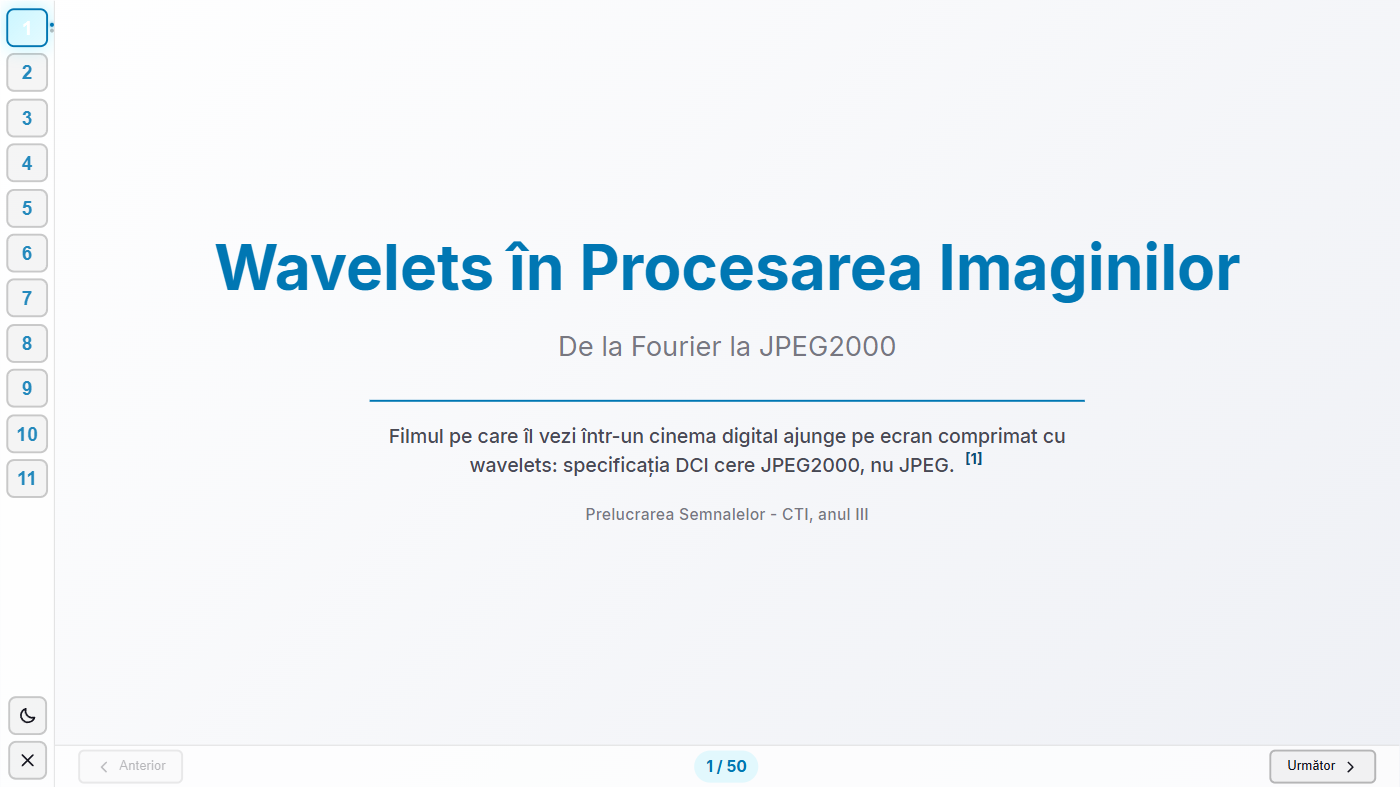
\includegraphics[width=\textwidth]{01-intro-title.png}
\caption{Ecranul de deschidere al turului: cârligul leagă subiectul de o
  cerință de specificație reală. Cinematograful digital impune JPEG2000 în
  locul lui JPEG, prin specificația DCI~\cite{dci2024}.}
\label{fig:intro-title}
\end{figure}

\begin{figure}[htbp]
\centering
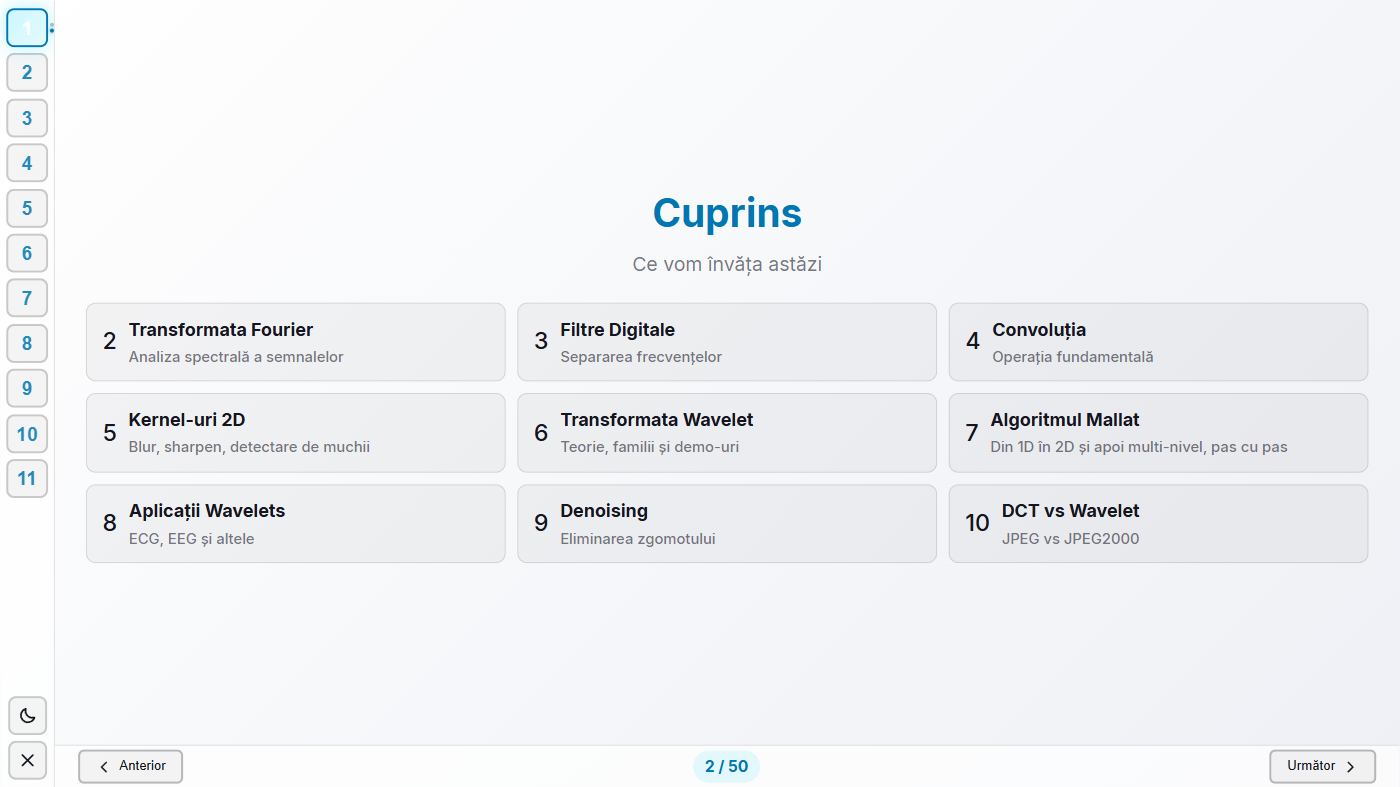
\includegraphics[width=\textwidth]{02-intro-toc.png}
\caption{Cuprinsul turului: nouă secțiuni, cu carduri clickabile care sar
  direct la secțiunea aleasă.}
\label{fig:intro-toc}
\end{figure}

\section{Harta: de la ecran la capitol}
\label{sec:harta}

Prezentarea are cincizeci de ecrane, numerotate în bara de jos a aplicației.
Tabelul~\ref{tab:harta} spune, pentru fiecare grup de ecrane, unde se citește
aceeași materie în textul de față. Citit invers, spune ce ecran să deschizi
pentru un capitol anume.

\begin{table}[htbp]
\centering
\caption{Corespondența dintre ecranele turului și capitolele acestui text.}
\label{tab:harta}
\small
\begin{tabular}{@{}llp{5.3cm}@{}}
\toprule
Ecrane & Secțiunea din tur & Unde se citește \\
\midrule
1--2 & Deschidere, cuprins & Capitolul~\ref{ch:intro} \\
3--5 & Transformata Fourier & Capitolul~\ref{ch:fundamente} \\
6--9 & Filtre digitale & Secțiunea~\ref{sec:filtre} \\
10--13 & Convoluția & Capitolul~\ref{ch:fundamente} \\
14--16 & Kernel-uri 2D & Secțiunea~\ref{sec:kernele} \\
17--24 & Transformata wavelet & Capitolul~\ref{ch:wavelets} \\
25--32 & Algoritmul lui Mallat & Secțiunea~\ref{sec:mallat} \\
33--35 & Aplicații, ECG & Capitolul~\ref{ch:ecg} \\
36--37 & EEG & Capitolul~\ref{ch:eeg} \\
38--39 & Amprenta audio & Capitolul~\ref{ch:shazam} \\
40--42 & Denoising & Capitolul~\ref{ch:denoising} \\
43--47 & DCT față de wavelet & Capitolul~\ref{ch:compresie} \\
48--50 & Sinteză, bibliografie & Capitolul~\ref{ch:sinteza} \\
\bottomrule
\end{tabular}
\end{table}

Capitolul~\ref{ch:tehnic} nu are ecrane proprii: descrie cum este construită
și verificată aplicația.

\chapter{Fourier, filtre și convoluție: instrumentele de bază}
\label{ch:fundamente}

Restul documentului se sprijină pe trei idei simple, în ordine: orice semnal
e o sumă de frecvențe, un filtru alege care dintre ele rămân, iar convoluția
e mecanismul care face asta. Wavelets, câteva capitole mai încolo, e ce se
întâmplă când combini toate trei cu o singură idee nouă.

\section{Transformata Fourier}

Shazam recunoaște o piesă din zece secunde de audio pentru că amprenta ei de
frecvențe e unică~\cite{wang2003}, adică exact amprenta pe care o calculează
transformata Fourier (revenim pe larg la Shazam în
Capitolul~\ref{ch:shazam}). Rezultatul central al transformatei e că orice
semnal se scrie ca o sumă, sau pentru semnale continue o integrală, de
sinusoide~\cite{lyons2011}:
\[
F(\omega) = \int_{-\infty}^{\infty} f(t)\,e^{-i\omega t}\,dt, \qquad
f(t) = \frac{1}{2\pi}\int_{-\infty}^{\infty} F(\omega)\,e^{i\omega t}\,d\omega,
\]
unde pulsația $\omega = 2\pi f$ e aceeași mărime ca frecvența $f$, doar în alte
unități (rad/s față de Hz). Formula lui Euler, $e^{i\theta} = \cos\theta +
i\sin\theta$, e ce leagă exponențiala complexă de sinusoide. Teorema lui
Parseval,
\[
\int_{-\infty}^{\infty} |f(t)|^2\,dt = \frac{1}{2\pi}\int_{-\infty}^{\infty} |F(\omega)|^2\,d\omega,
\]
spune că energia semnalului e aceeași, calculată în timp sau în frecvență. E o
proprietate la care revenim când arătăm că nici transformata wavelet
discretă nu pierde energie.

Limita transformatei contează la fel de mult ca rezultatul: Fourier spune CE
frecvențe conține un semnal, dar nu CÂND apar ele. Un mashup din două piese
are, pe porțiuni lungi, un spectru foarte asemănător cu suprapunerea lor,
tocmai de-aceea Shazam rulează transformata pe ferestre scurte și succesive,
nu pe piesa întreagă (transformata Fourier pe termen scurt, STFT).
Fereastra scurtă fixează unde se pierde: cu cât fereastra e mai scurtă, cu
atât localizarea în timp e mai bună și rezoluția în frecvență mai slabă,
exact compromisul pe care wavelets îl rezolvă altfel, cu ferestre de
dimensiune variabilă (Capitolul~\ref{ch:wavelets}).

Demo-ul din tur (Figura~\ref{fig:fourier-demo}) calculează efectiv o
transformată Fourier rapidă (\txt{np.fft.fft}) pentru opt funcții
predefinite: sinusoidă simplă, două și trei frecvențe, chirp, puls
Gaussian, undă pătrată, suma Fourier a undei pătrate și o expresie
personalizată, evaluată printr-o listă restrânsă de funcții permise
(\txt{sin}, \txt{cos}, \txt{exp}, \txt{pi}, \txt{abs}, \txt{sqrt}). Afișează
simultan domeniul timp și spectrul de magnitudine.

Presetul cu suma Fourier a undei pătrate arată o limită care revine mai
târziu. Cu fiecare armonică adăugată suma se apropie de unda pătrată, dar
lângă discontinuitate rămâne o supraoscilație de aproape nouă la sută din
saltul semnalului. Ea se îngustează pe măsură ce adaugi termeni și nu scade
niciodată în înălțime. Fenomenul poartă numele lui Gibbs și e ce se întâmplă
ori de câte ori tai brusc un spectru. Pentru presetul
din figură, $f(t) = \sin(2\pi \cdot 5 t) + \sin(2\pi \cdot 12 t)$, cele două
vârfuri spectrale cad exact la 5 și 12~Hz.

\begin{figure}[htbp]
\centering
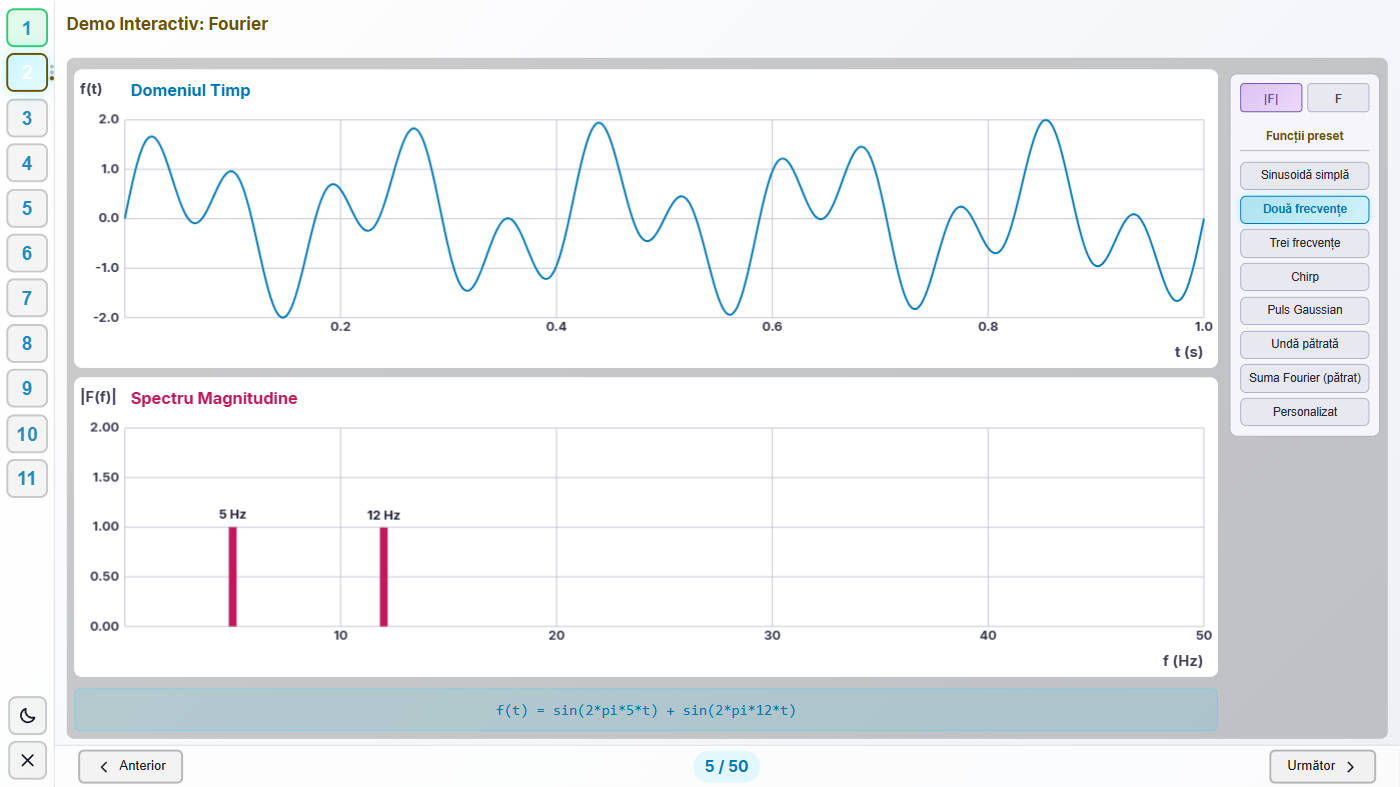
\includegraphics[width=\textwidth]{05-fourier-demo.png}
\caption{Domeniul timp și spectrul de magnitudine calculate live pentru
  presetul „Două frecvențe”: vârfurile spectrale cad exact la 5 și 12~Hz,
  frecvențele din formula afișată dedesubt.}
\label{fig:fourier-demo}
\end{figure}

\section{Filtre digitale}
\label{sec:filtre}

Un filtru păstrează o parte din spectru și atenuează restul, teoria
standard de proiectare a filtrelor digitale~\cite{oppenheimschafer2010}.
Trei forme apar în tur, toate normalizate să treacă prin $-3$~dB (adică
$|H|=1/\sqrt2$, jumătate din putere) exact la frecvența de tăiere $f_c$, ca
să fie comparabile la aceeași tăietură:
\begin{gather*}
H^{\text{ideal}}_{LP}(f) = \begin{cases} 1 & |f|\le f_c \\ 0 & |f| > f_c \end{cases} \\[4pt]
\left|H^{\text{Butterworth}}_{LP}(f)\right|^2 = \frac{1}{1+\left(f/f_c\right)^{2n}} \\[4pt]
H^{\text{Gaussian}}_{LP}(f) = e^{-\frac{\ln 2}{2}\left(f/f_c\right)^2}
\end{gather*}
Filtrul ideal are un prag dur chiar la $f_c$, imposibil de realizat în
practică: răspunsul lui în timp e un \emph{sinc} infinit, deci necauzal, iar
trunchierea lui readuce oscilația Gibbs întâlnită deja la Fourier. Butterworth
și Gaussian sunt calibrate să dea exact $|H|^2=\tfrac12$ la $f=f_c$, oricare
ar fi ordinul $n$ sau lățimea Gaussianei. Ordinul controlează doar cât de
abrupt coboară restul curbei, de la $n=1$ (lent) la $n=8$ (aproape ideal).
Varianta trece-sus e complementul în putere al variantei trece-jos,
\[
H_{HP}(f) = \sqrt{1-\left|H_{LP}(f)\right|^2}, \qquad
\text{deci} \quad |H_{LP}|^2+|H_{HP}|^2=1
\]
la orice frecvență: cele două filtre împart mereu toată puterea, indiferent
de formă sau ordin. Varianta trece-bandă înlănțuie un trece-sus la tăietura
joasă cu un trece-jos la tăietura înaltă, $H_{BP}(f) =
\sqrt{1-|H_{LP}(f;f_{lo})|^2}\cdot H_{LP}(f;f_{hi})$.

\begin{figure}[htbp]
\centering
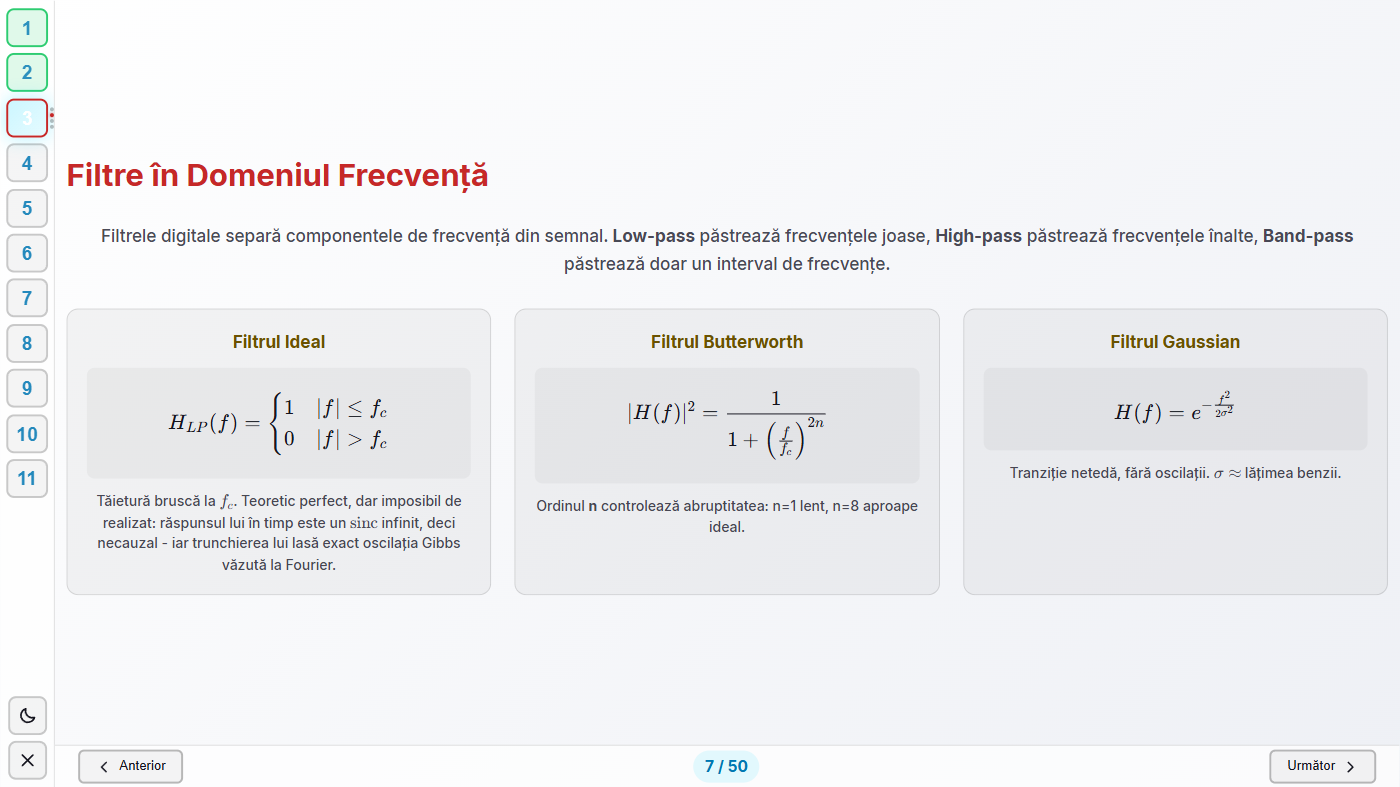
\includegraphics[width=\textwidth]{07-filters-theory.png}
\caption{Cele trei forme ale filtrului trece-jos, toate normalizate la
  $-3$~dB pe frecvența de tăiere $f_c$.}
\label{fig:filters-theory}
\end{figure}

În back-end, o singură funcție, \txt{filter_magnitude}, produce atât curba
de răspuns desenată pe ecran (Figura~\ref{fig:filters-demo}), cât și
multiplicatorul aplicat efectiv semnalului: cererea
\txt{/api/filters/apply-signal} transformă semnalul cu FFT, îl înmulțește cu
acel multiplicator și aplică FFT inversă. Multiplicatorul e real și par în
frecvență, așa că semnalul filtrat rămâne real și filtrul e zero-fază. Iar
faptul că e o singură funcție înseamnă că demo-ul nu poate afișa un filtru
și calcula altul, o clasă întreagă de bug posibil eliminată prin construcție.

\begin{figure}[htbp]
\centering
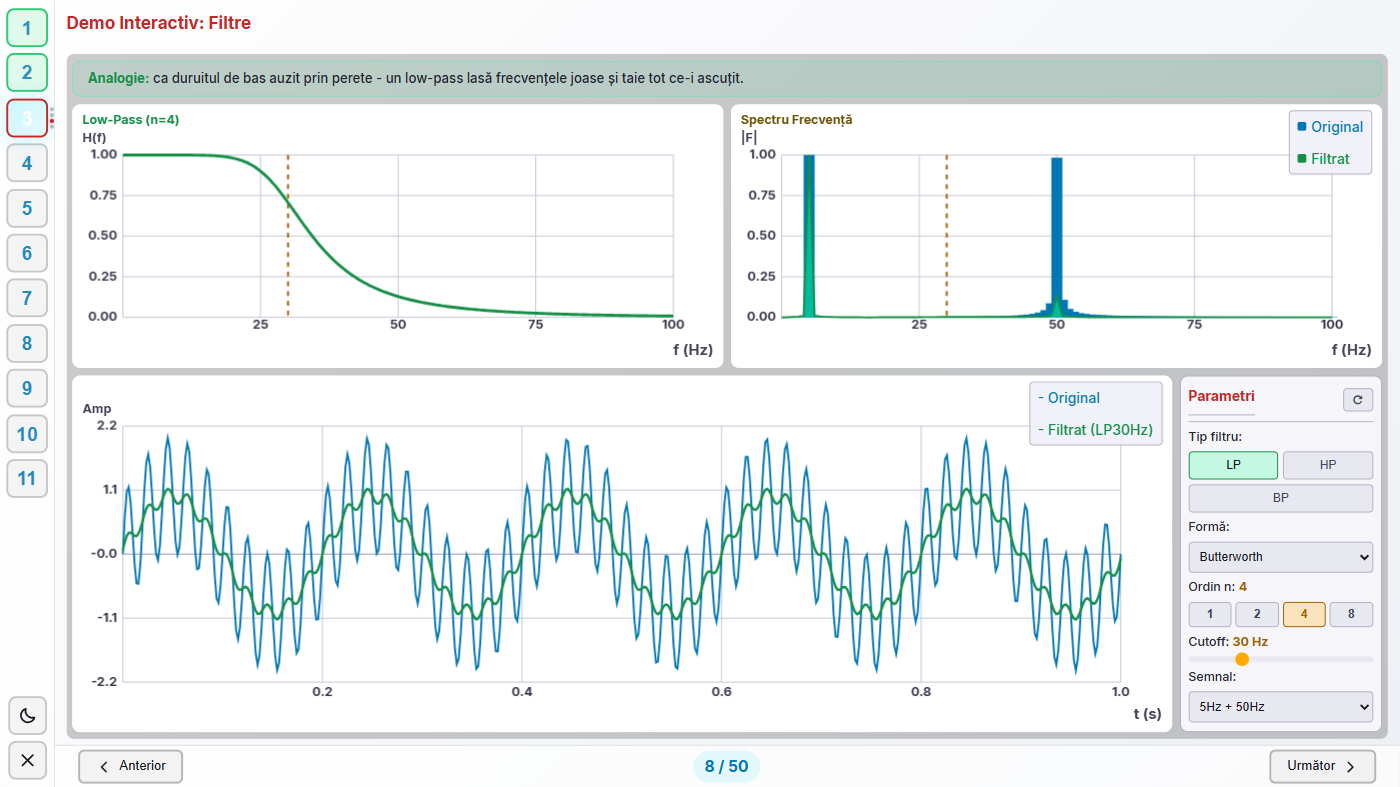
\includegraphics[width=\textwidth]{08-filters-demo.png}
\caption{Filtru trece-jos Butterworth de ordinul 4: răspunsul în frecvență
  (stânga sus), spectrul semnalului înainte și după filtrare (dreapta sus) și
  semnalul filtrat în timp (jos), toate recalculate la orice schimbare de
  parametru.}
\label{fig:filters-demo}
\end{figure}

Băncile de filtre, cu un trece-jos $h$ pentru coeficienți de aproximare și un
trece-sus $g$ pentru coeficienți de detaliu, aplicate recursiv, dau analiza
multi-rezoluție~\cite{strangnguyen1996}, punctul de plecare al
Capitolului~\ref{ch:wavelets}. Condiția care garantează reconstrucție
perfectă e relația de filtre-oglindă-conjugate,
$g[k] = (-1)^k h[N-1-k]$~\cite{estebangaland1977,smithbarnwell1984}, iar
motivul pentru care decimarea cu doi după fiecare filtrare nu pierde
informație vine direct din teorema eșantionării: o bandă de $B$~Hz cere
doar $2B$ eșantioane pe secundă~\cite{shannon1949}, exact atât cât rămâne
după ce fiecare filtru înjumătățește banda.

\section{Convoluția}

Definiția 1D, $(f*g)[n] = \sum_k f[k]\,g[n-k]$, stă la baza filtrelor de mai
sus și a rețelelor convoluționale deopotrivă. Teorema convoluției,
$f*g \leftrightarrow F\cdot G$~\cite{lyons2011}, leagă cele două: o
convoluție în timp e o simplă înmulțire în frecvență, motivul pentru care
FFT reduce complexitatea unei convoluții lungi de la $O(n^2)$ la
$O(n\log n)$: transformi, înmulțești punct cu punct, transformi înapoi.

Extensia la imagini,
\[
(I*K)[x,y] = \sum_{i,j} I[x-i,\,y-j]\cdot K[i,j],
\]
rotește kernelul cu $180^\circ$ (semnele minus). Bibliotecile de procesare
de imagini, și demo-urile din tur, calculează de fapt \emph{corelație}, cu
$I[x+i,y+j]$, fără rotația kernelului: pentru kernele simetrice (blur,
Gaussian, Laplacian) rezultatul e identic, iar diferența apare doar la
kernele asimetrice, la Sobel de exemplu, unde rotația ar inversa semnul
gradientului (Figura~\ref{fig:conv-2d}).

\begin{figure}[htbp]
\centering
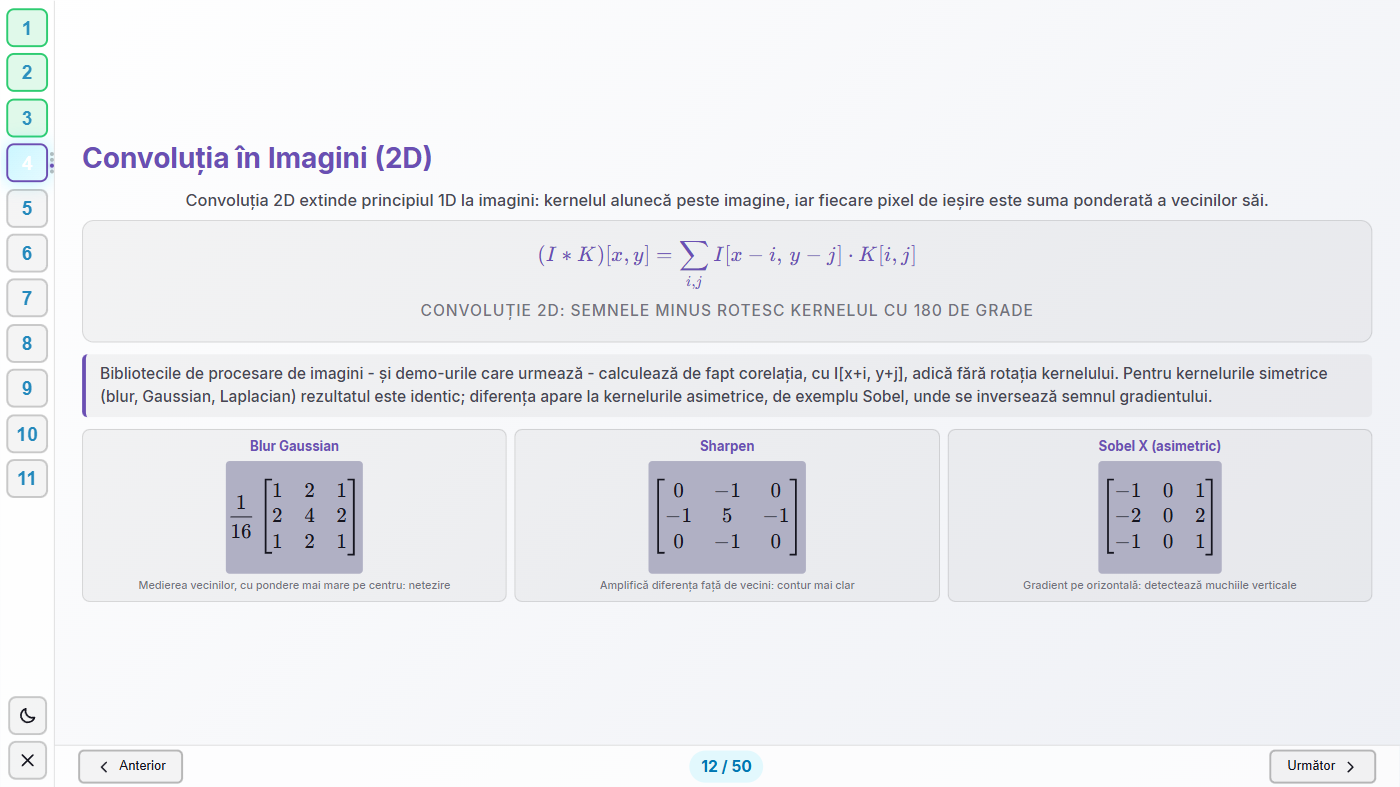
\includegraphics[width=\textwidth]{12-conv-2d.png}
\caption{Convoluția 2D cu semnul corect și nota despre corelație versus
  convoluție, alături de trei kernele reprezentative: blur Gaussian, sharpen
  și Sobel X (asimetric).}
\label{fig:conv-2d}
\end{figure}

\section{Fourier în două dimensiuni}
\label{sec:fourier-2d}

Înainte de a trece la kernele, turul face un pas lateral care merită explicat,
pentru că e locul unde tot ce s-a spus despre semnale 1D se mută pe imagini.
Transformata Fourier discretă se aplică la fel de bine unei matrice de pixeli,
pe rânduri și apoi pe coloane, iar rezultatul e tot o matrice, de aceeași
dimensiune, pe care o vedem ca imagine: spectrul de magnitudine
(Figura~\ref{fig:sound-to-image}). Backend-ul o calculează la cerere, prin
\txt{/api/fourier/image}, pe imaginea aleasă din listă.

Se citește altfel decât un spectru 1D. Frecvențele joase stau în centru, cele
înalte spre margini, iar distanța față de centru înseamnă cât de repede se
schimbă intensitatea, nu unde se întâmplă schimbarea. O zonă întinsă și
uniformă, cerul sau un perete, produce energie concentrată în centru. Muchiile și
textura fină împing energie spre margini, iar orientarea se păstrează: o
textură cu dungi verticale lasă o urmă orizontală în spectru, perpendiculară
pe dungi. Scara e logaritmică, altfel componenta continuă din centru ar fi
singurul lucru vizibil.

Consecința practică leagă capitolul: un blur de telefon e un filtru trece-jos
în două dimensiuni, iar o accentuare de contur e un trece-sus, exact aceleași
două operații din Secțiunea~\ref{sec:filtre}, doar că acum tăietura se face pe
un disc în jurul centrului, nu pe un interval de pe o axă. Kernelele din
secțiunea următoare sunt fix aceste filtre, scrise în domeniul spațial.

\begin{figure}[htbp]
\centering
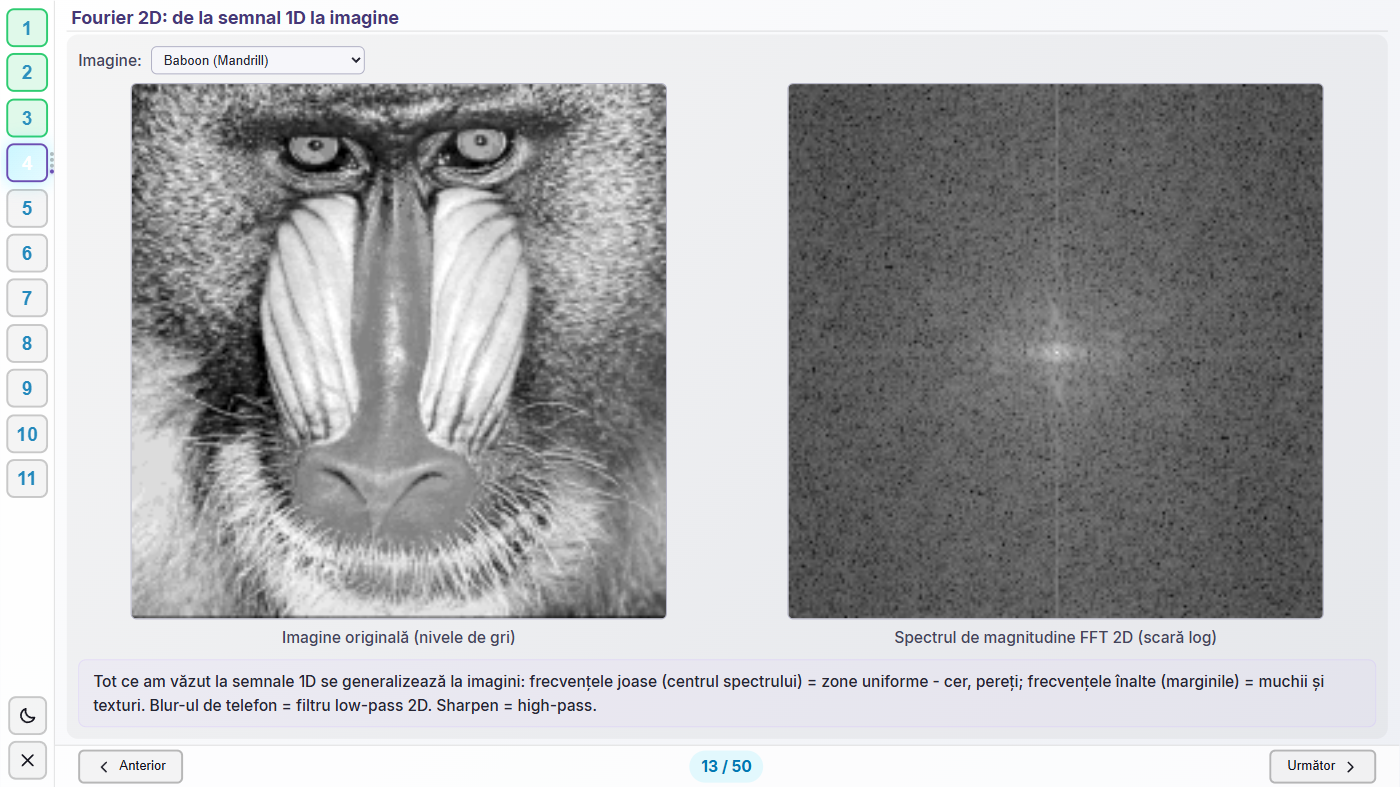
\includegraphics[width=\textwidth]{13-sound-to-image.png}
\caption{Aceeași imagine în cele două domenii: originalul în nivele de gri
  (stânga) și spectrul lui de magnitudine 2D pe scară logaritmică (dreapta),
  cu frecvențele joase în centru. Blana deasă a babuinului umple spectrul spre
  margini, semnătura unei texturi fine.}
\label{fig:sound-to-image}
\end{figure}

\section{Kernele 2D, pe familii}
\label{sec:kernele}

Un demo educațional descompune aplicarea unui kernel pas cu pas, cu fereastra
care alunecă, produsul element-cu-element și suma, înainte de a trece la
kernele aplicate pe imagini reale (Figura~\ref{fig:kernels-demo}): blur
(cutie sau Gaussian), ascuțire (normală sau puternică), detectare de muchii
(Laplacian, Laplacian diagonal, Sobel, Prewitt, contur) și emboss, fiecare
cu raza (3, 4 sau 5) și puterea efectului reglabile independent.

\begin{figure}[htbp]
\centering
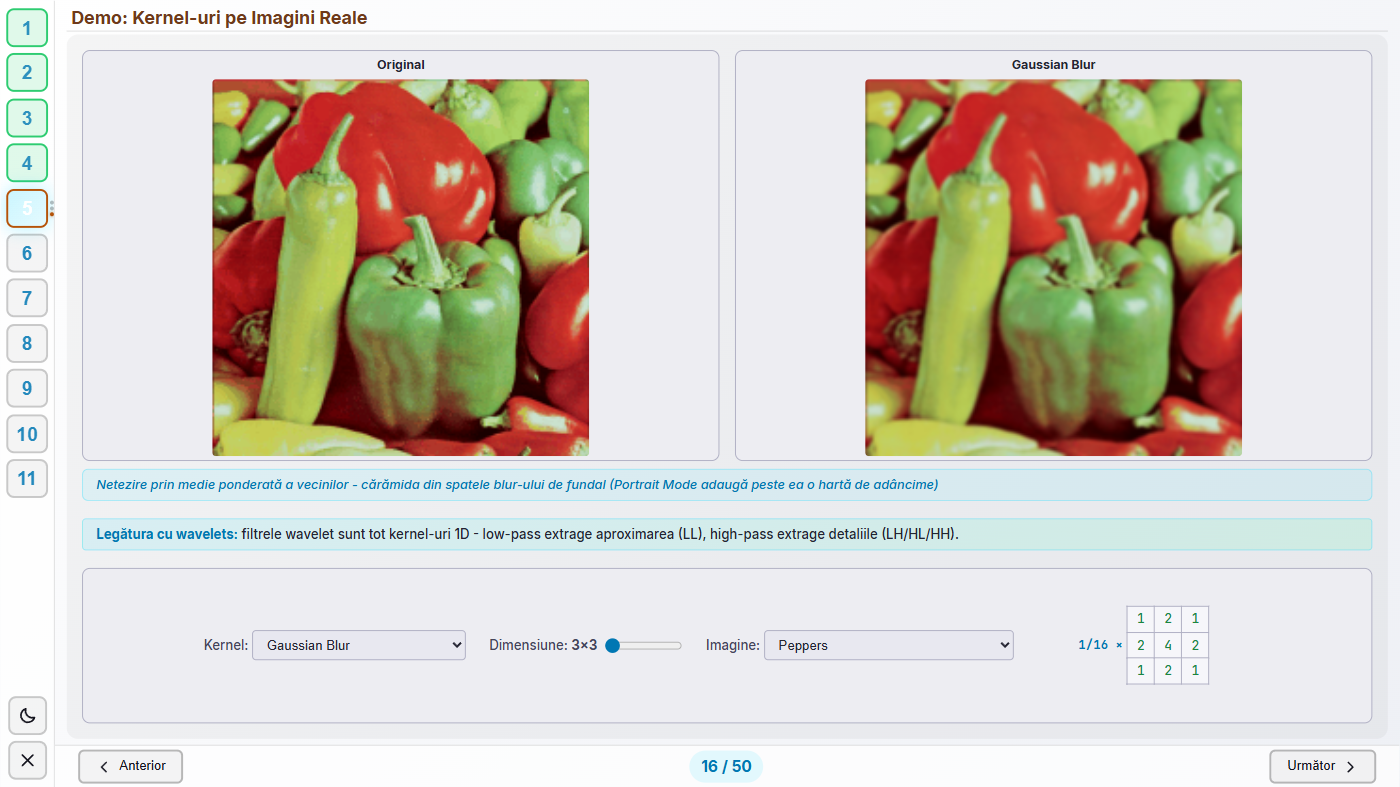
\includegraphics[width=\textwidth]{16-kernels-demo.png}
\caption{Blur Gaussian $3\times 3$ aplicat pe imaginea Peppers, cu matricea
  de kernel afișată exact așa cum e trimisă către back-end.}
\label{fig:kernels-demo}
\end{figure}

Redimensionarea unui kernel la o rază mai mare trebuie să păstreze \emph{ce
face} kernelul, nu doar dimensiunea lui, iar o singură regulă nu ajunge
pentru toate familiile. Identitatea rămâne o deltă discretă la orice
dimensiune. Kernele de blur adevărat (toate valorile nenegative, suma 1)
devin cutie sau Gaussian, după cum sursa era uniformă sau nu. Kernele de
muchie (suma 0) păstrează tiparul $3\times 3$ pe inelul exterior și
rebalansează centrul ca suma să rămână 0 la orice dimensiune. Kernele
direcționale (emboss) sunt interpolate biliniar și rescalate ca să
păstreze suma originală, care le fixează luminozitatea rezultatului. Kernele
de ascuțire simetrică, cu suma 1 dar și valori negative, deci nu blur, se
reconstruiesc ca \emph{unsharp masking} la noua rază,
\[
K_{\text{sharpen}}(r) = (1+\alpha)\,\delta_r - \alpha\, G_r,
\]
unde $\delta_r$ e delta discretă, $G_r$ Gaussiana normalizată la raza $r$,
iar $\alpha$ vine din valoarea centrală a kernelului original minus 1, ca un
sharpen la $3\times 3$ și unul la $5\times 5$ să păstreze aceeași putere a
efectului.

Distincția pe familii a intrat în cod după ce o regulă mai simplă,
„orice kernel cu suma 1 e un blur”, s-a dovedit greșită: și ascuțirea, și
emboss-ul, și identitatea au suma 1, așa că un „Sharpen” cerut la
$5\times 5$ întorcea de fapt o gaussiană, cu un câștig măsurat de zero la
frecvența Nyquist. Cu funcția rescrisă pe familii, pe o fotografie reală,
varianța laplacianului imaginii, o măsură standard de claritate, urcă de
la 2307 pe original la 40150, 33893 și respectiv 32114 pentru ascuțire la
$3\times 3$, $5\times 5$ și $7\times 7$.

\chapter{Transformata wavelet și algoritmul lui Mallat}
\label{ch:wavelets}

\section{De ce wavelets}

La un cutremur, unda P sosește la $t=12$s și unda S la $t=38$s. Un spectru
Fourier calculat pe tot semnalul nu poate spune când s-a schimbat regimul,
ceea ce lipsește e localizarea. Wavelets rezolvă exact asta: în loc de o
sinusoidă infinită, folosesc un „wavelet mamă” $\psi$, o undă scurtă, cu
energie concentrată local, scalată și translatată,
\[
\psi_{a,b}(t) = \frac{1}{\sqrt{|a|}}\,\psi\!\left(\frac{t-b}{a}\right),
\]
unde $b$ e momentul de timp și $a$ scala, invers proporțională cu
frecvența, deci $a$ mic prinde detalii de frecvență înaltă, $a$ mare prinde
structuri de frecvență joasă. Rezultatul e o analiză multi-rezoluție:
semnale nestaționare (muzică, ECG, cutremure) capătă o descriere în care
timpul și frecvența apar simultan.

Compromisul e formalizat de principiul de incertitudine al lui Heisenberg,
$\Delta t \cdot \Delta f \ge 1/(4\pi)$~\cite{mallat2008}: fiecare metodă
împarte planul timp-frecvență în dreptunghiuri de arie constantă, dar forma
lor diferă. Fourier pur dă rezoluție infinită în frecvență și nulă în timp.
STFT, cu fereastră fixă, dă un compromis identic la orice frecvență.
Wavelets adaptează fereastra: îngustă în timp la frecvențe înalte, îngustă
în frecvență la frecvențe joase (Figura~\ref{fig:heisenberg-scalogram},
stânga), forma care se potrivește cel mai bine cu semnale reale, unde
tranzițiile scurte (un atac de tobă, un complex QRS) coexistă cu structuri
lungi (un bas continuu, linia de bază a unui ECG).

Scalograma (Figura~\ref{fig:heisenberg-scalogram}, dreapta) arată aceeași
idee pe un semnal concret: transformata wavelet continuă a unui chirp
modulat în amplitudine produce o bandă diagonală, frecvența crește cu
timpul, a cărei intensitate urmărește chiar amplitudinea semnalului de
intrare.

\begin{figure}[htbp]
\centering
\begin{subfigure}[t]{0.485\textwidth}
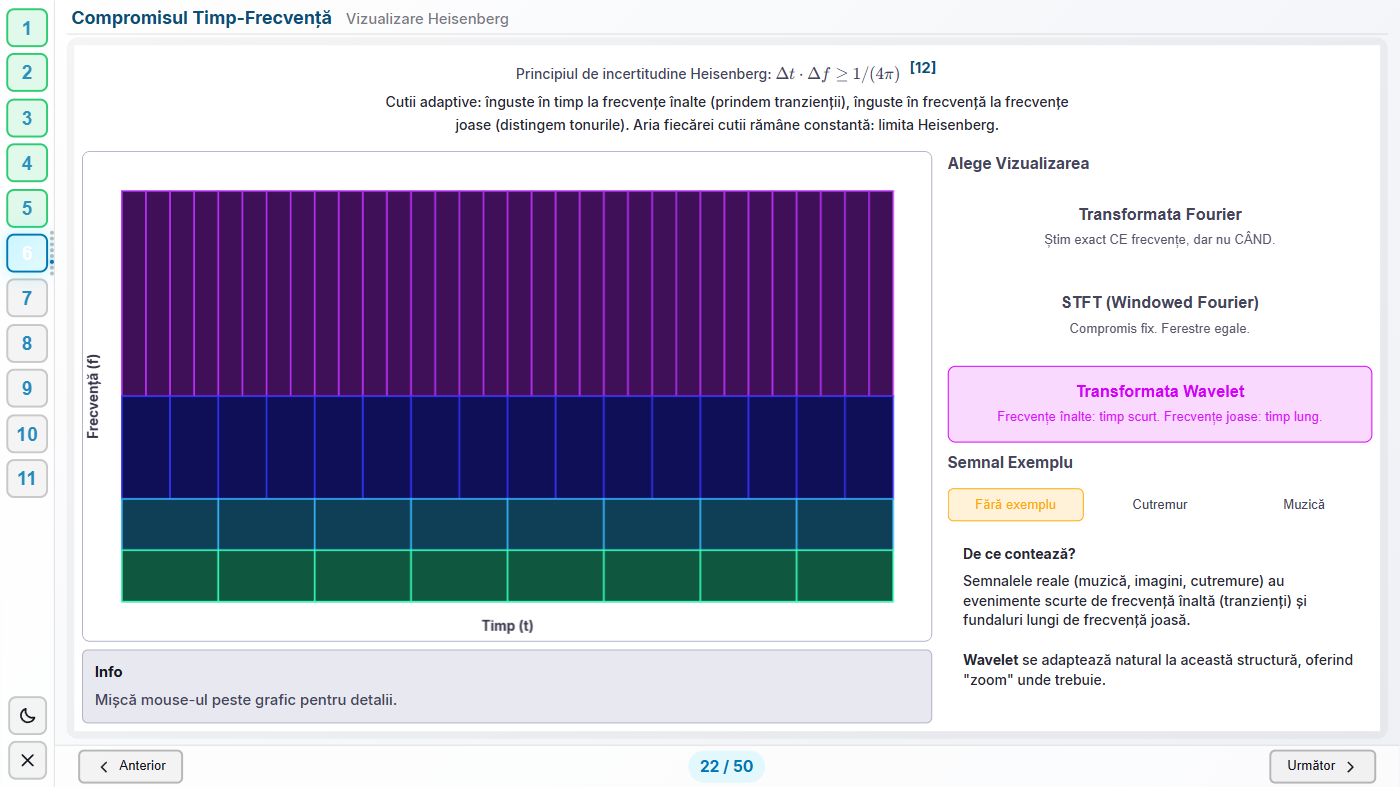
\includegraphics[width=\textwidth]{22-heisenberg-boxes.png}
\caption{Cutii de arie constantă: înguste în timp la frecvențe înalte, înguste
  în frecvență la frecvențe joase.}
\end{subfigure}
\hfill
\begin{subfigure}[t]{0.485\textwidth}
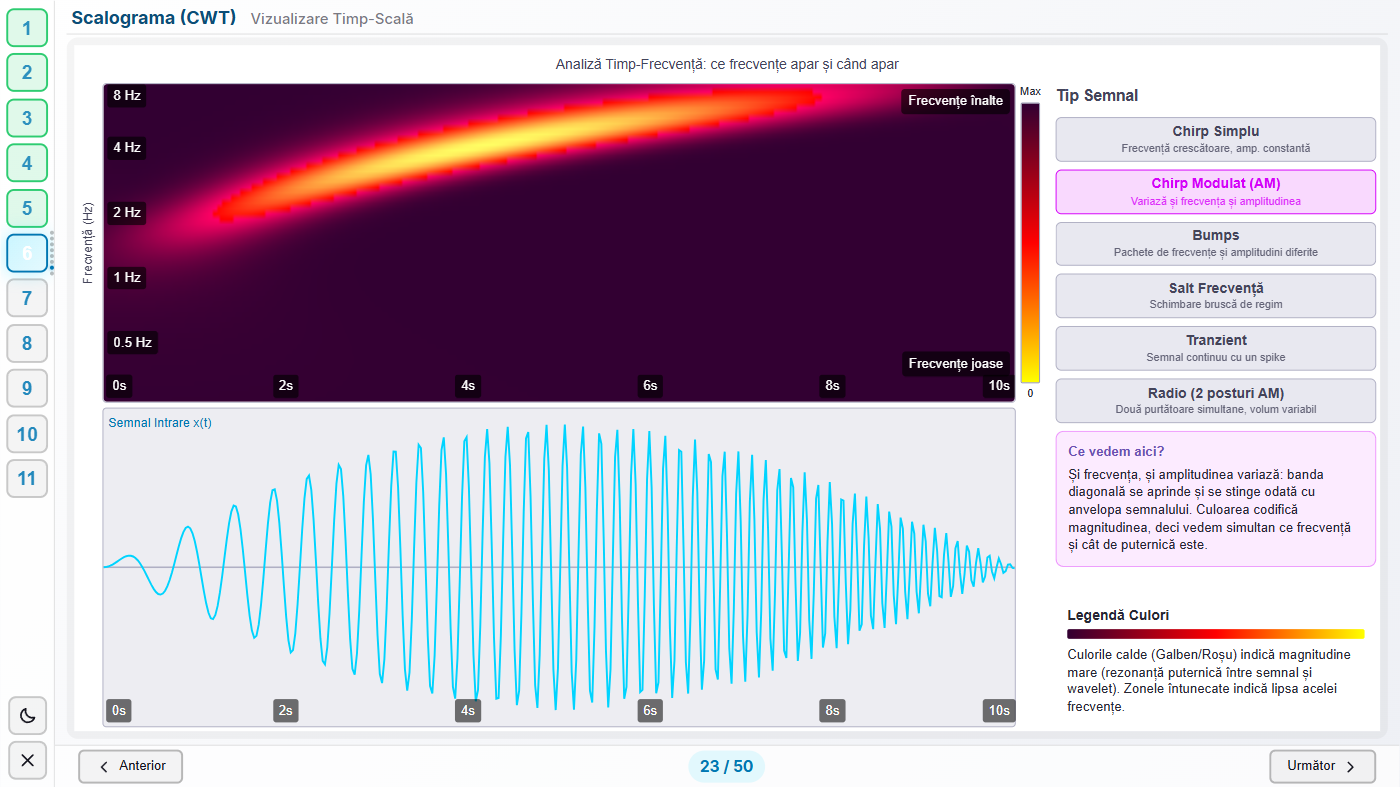
\includegraphics[width=\textwidth]{23-scalogram.png}
\caption{Scalograma unui chirp modulat: banda diagonală urcă în frecvență și
  respiră odată cu amplitudinea.}
\end{subfigure}
\caption{Compromisul timp-frecvență, teoretic (stânga) și pe un semnal
  concret (dreapta).}
\label{fig:heisenberg-scalogram}
\end{figure}

\section{Familii de wavelets}

Nu orice undă scurtă e un wavelet valid. Condiția de admisibilitate cere ca
$\int_0^\infty |\hat\psi(\omega)|^2/\omega\,d\omega$ să fie finită, ceea ce
pentru un $\psi$ integrabil forțează media lui nulă,
$\int \psi(t)\,dt = 0$~\cite{daubechies1992}, de-aici numele de familie: un
wavelet oscilează în jurul lui zero, nu se așază pe o valoare. Funcția de
scalare $\phi$ și wavelet-ul $\psi$ se leagă recursiv prin coeficienții
filtrului,
\[
\phi(t) = \sqrt2\sum_k h_k\,\phi(2t-k), \qquad
\psi(t) = \sqrt2\sum_k g_k\,\phi(2t-k),
\]
cu $g$ obținut din $h$ prin aceeași relație de filtre-oglindă-conjugate din
Secțiunea~\ref{sec:filtre}~\cite{estebangaland1977,smithbarnwell1984}.
Familia Daubechies~\cite{daubechies1988}, Symlet, Coiflet, Morlet și altele
diferă prin numărul de coeficienți și prin cât de simetrice sunt, toate
schimbă doar $\phi$ și $\psi$, algoritmul de mai jos rămâne același.

Transformata continuă, $W(a,b) = \int f(t)\cdot\frac{1}{\sqrt a}\psi^*
\left(\frac{t-b}{a}\right)dt$, evaluează $(a,b)$ pe un continuu, deci
informația se repetă. Transformata discretă eșantionează diadic, $a=2^j$,
$b=k\cdot 2^j$, și produce exact atâția coeficienți câți sunt necesari
pentru o bază ortonormală, fără redundanță~\cite{mallat2008}, baza pe care
lucrează algoritmul lui Mallat, mai jos. Un demo din tur desenează live
forma mamă pentru orice familie disponibilă în PyWavelets, citind direct
rezultatul funcției \txt{wavefun()} a bibliotecii. O sinusoidă simplă e
inclusă explicit ca ne-exemplu, fiindcă n-are nicio localizare în timp, deci
nu e wavelet.

\begin{figure}[htbp]
\centering
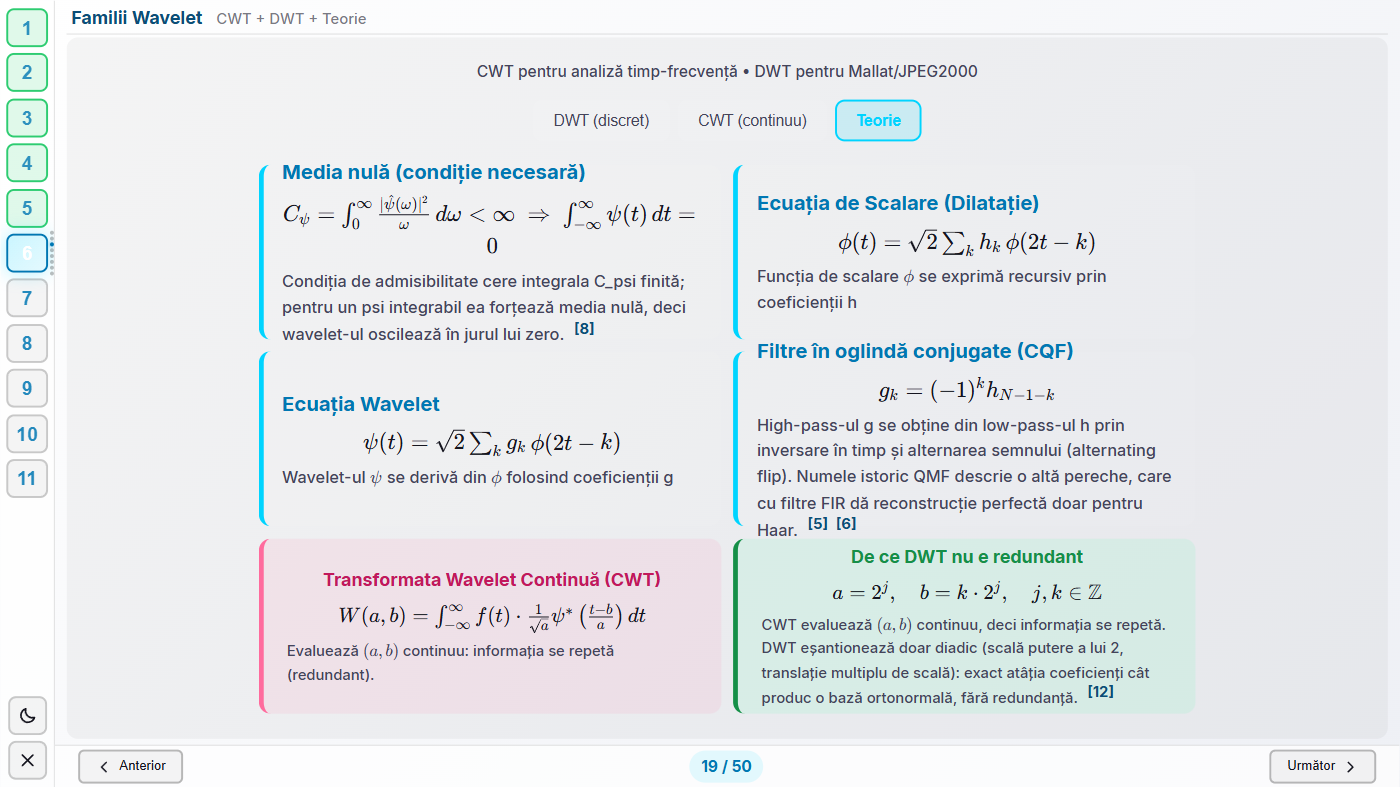
\includegraphics[width=\textwidth]{19-wavelet-families.png}
\caption{Cele patru rezultate din spatele familiilor wavelet: media nulă,
  ecuațiile de scalare/wavelet, perechea CQF și non-redundanța DWT, fiecare cu
  citarea lui.}
\label{fig:wavelet-families}
\end{figure}

\section{Wavelet-ul complex și faza}
\label{sec:complex}

Familiile de până acum sunt reale: un coeficient mare poate să însemne
rezonanță puternică, dar semnul lui depinde de unde anume a căzut wavelet-ul
peste oscilație. Mută semnalul cu o fracțiune de perioadă și coeficientul se
schimbă, deși conținutul nu s-a schimbat deloc. Wavelet-ul Morlet complex
rezolvă exact asta, pentru că e o gaussiană înmulțită cu o exponențială
complexă,
\[
  \psi(t) = e^{-t^2/2} \cdot e^{i\omega t}
          = e^{-t^2/2}\left(\cos(\omega t) + i \sin(\omega t)\right),
\]
adică două wavelet-uri reale defazate cu un sfert de perioadă, folosite
împreună. Coeficientul devine un număr complex, din care se citesc separat
magnitudinea, care spune \emph{cât} de puternică e rezonanța și nu se mai
schimbă la deplasarea semnalului, și faza, care spune \emph{unde} a căzut
oscilația în interiorul ferestrei.

Ecranul din tur (Figura~\ref{fig:complex-wavelet}) arată wavelet-ul ca o
spirală în trei dimensiuni: timpul pe o axă, partea reală pe a doua, partea
imaginară pe a treia, cu culoarea codificând faza de la $-\pi$ la $\pi$.
Proiecția pe fiecare perete dă cele două componente reale, iar spirala e
motivul pentru care scalograma din secțiunea anterioară arată benzi netede și
nu o alternanță de dungi luminoase și întunecate: acolo se desenează
magnitudinea coeficientului complex, care nu depinde de fază.

Aceeași proprietate e motivul pentru care wavelet-urile complexe se folosesc
la detectarea trăsăturilor invariante la translație și la analiza mișcării,
unde contează ce s-a întâmplat, nu la ce microsecundă a căzut fereastra.

\begin{figure}[htbp]
\centering
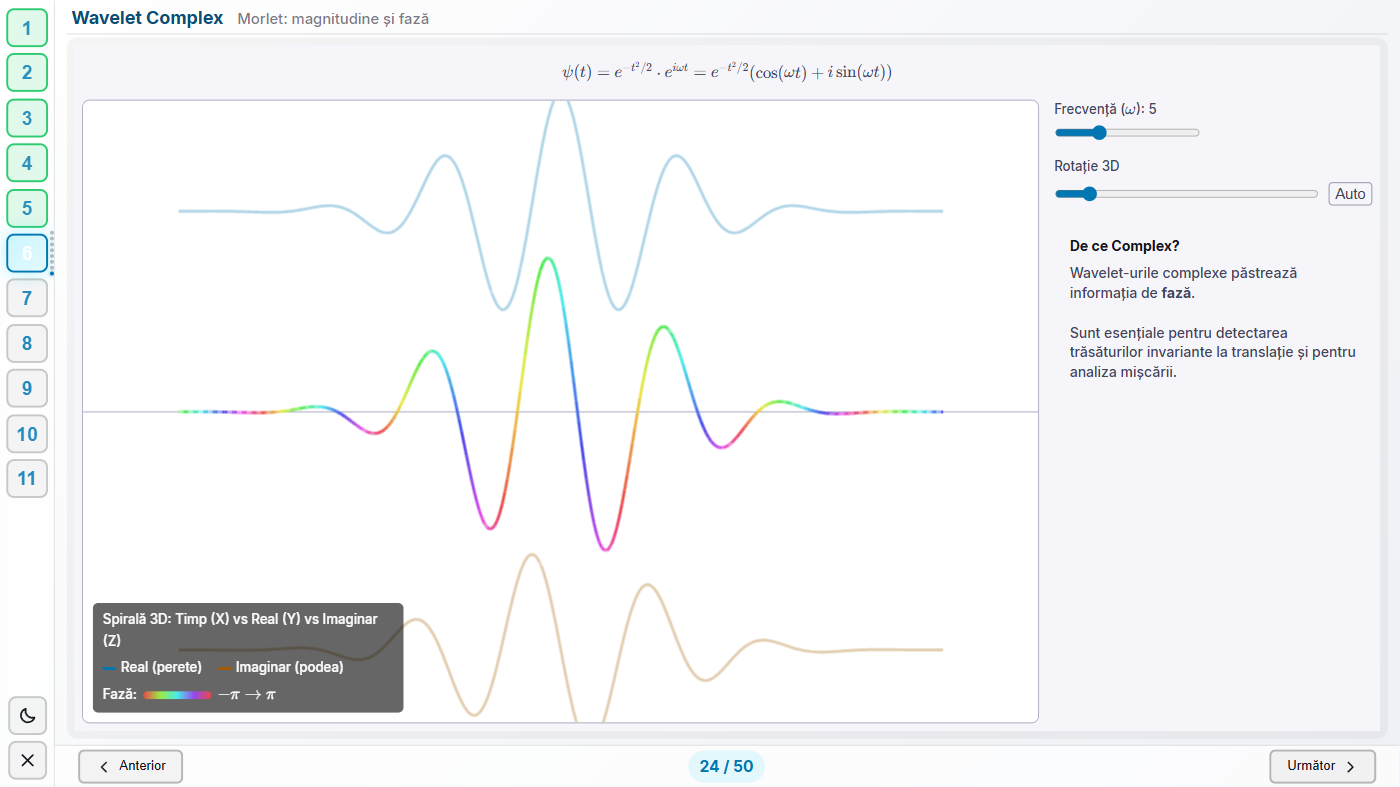
\includegraphics[width=\textwidth]{24-complex-wavelet.png}
\caption{Wavelet-ul Morlet complex ca spirală: partea reală proiectată pe un
  perete, partea imaginară pe celălalt, iar culoarea curbei centrale codifică
  faza. Frecvența și unghiul de rotație sunt reglabile din dreapta.}
\label{fig:complex-wavelet}
\end{figure}

\section{Algoritmul lui Mallat}
\label{sec:mallat}

Formal, un semnal se descompune prin proiecție pe funcția de scalare și pe
wavelet la nivelul $j$,
\[
c_{j,k} = \int x(t)\,\phi_{j,k}(t)\,dt, \qquad d_{j,k} = \int x(t)\,\psi_{j,k}(t)\,dt.
\]
Contribuția lui Mallat e observația care face aceste integrale inutile de
calculat direct: coeficienții unui nivel se obțin din nivelul anterior doar
prin filtrare și decimare cu doi,
\[
c_{j+1,k} = \sum_n h_0[n-2k]\,c_{j,n}, \qquad
d_{j+1,k} = \sum_n h_1[n-2k]\,c_{j,n},
\]
unde $h_0$ e filtrul de aproximare $h$ și $h_1$ filtrul de detaliu $g$ din
ecuațiile de mai sus, scrise acum cu indici fiindcă apar împreună,
fără nicio integrală calculată efectiv~\cite{mallat1989,mallat2008}. E o
recursie exactă: fiecare nivel iese din cel anterior printr-o singură
trecere de filtrare, deci descompunerea pe $L$ niveluri costă $L$ perechi de
filtrări, nu $L$ integrale separate. În cod, aceeași recursie e
\txt{pywt.wavedec2(imagine, wavelet, level=niveluri)}, care întoarce
aproximarea cea mai grosieră plus câte un triplet de subbenzi de detaliu pe
nivel. Reconstrucția, \txt{pywt.waverec2}, trece coeficienții prin filtrele
de sinteză și îi însumează, operația inversă a celei de mai sus.

Pentru wavelet-ul Haar, singurul cu filtre de doi coeficienți, suma se scrie
pe un singur eșantion și devine o pereche de medie și diferență,
\[
x[2k] = \frac{cA[k]+cD[k]}{\sqrt2}, \qquad x[2k+1] = \frac{cA[k]-cD[k]}{\sqrt2},
\]
forma folosită de demo-ul de reconstrucție din tur. Pentru orice filtru mai
lung, un Daubechies sau biortogonalul 9/7 din capitolul de compresie, un
eșantion reconstruit primește contribuții de la mai multe perechi
$(cA,cD)$ vecine, iar formula de mai sus nu se mai aplică punct cu punct.

La imagini, aceeași pereche de filtre se aplică o dată pe rânduri și o dată
pe coloane, dând patru subbenzi, $LL$ (aproximare), $LH$/$HL$ (detalii
orizontale/verticale) și $HH$ (detalii diagonale). Analogia cu hărțile ajută:
la zoom mic vezi doar $LL$, structura globală. La zoom mare apar
$LH$/$HL$/$HH$, detaliile fine. Pasul se aplică recursiv doar pe $LL$.
High-pass pe coloane dă detalii \emph{orizontale} pentru că răspunde la
variația pe verticală, exact ce înseamnă o muchie orizontală.

Demo-ul educațional 1D (Figura~\ref{fig:mallat-1d-edu}) face vizibil un
nivel al algoritmului, pas cu pas, pe un semnal de 16 eșantioane, treaptă,
rampă, sinusoidă, puls sau o „melodie” de note discrete. Fereastra
filtrului, produsul și suma sunt animate explicit, apoi decimarea cu doi.
Interpretarea diferă cu forma semnalului, o treaptă produce un vârf de
detaliu exact la muchie, o melodie păstrează notele în aproximare și
marchează atacul fiecărei note în detaliu. Un glosar de notație, repetat pe
toate ecranele acestei secțiuni, ține evidența faptului că aceeași împărțire
circulă sub nume diferite în literatură și în cod: $c = cA = L = A$ pentru
aproximare, $d = cD = H = D$ pentru detaliu.

\begin{figure}[htbp]
\centering
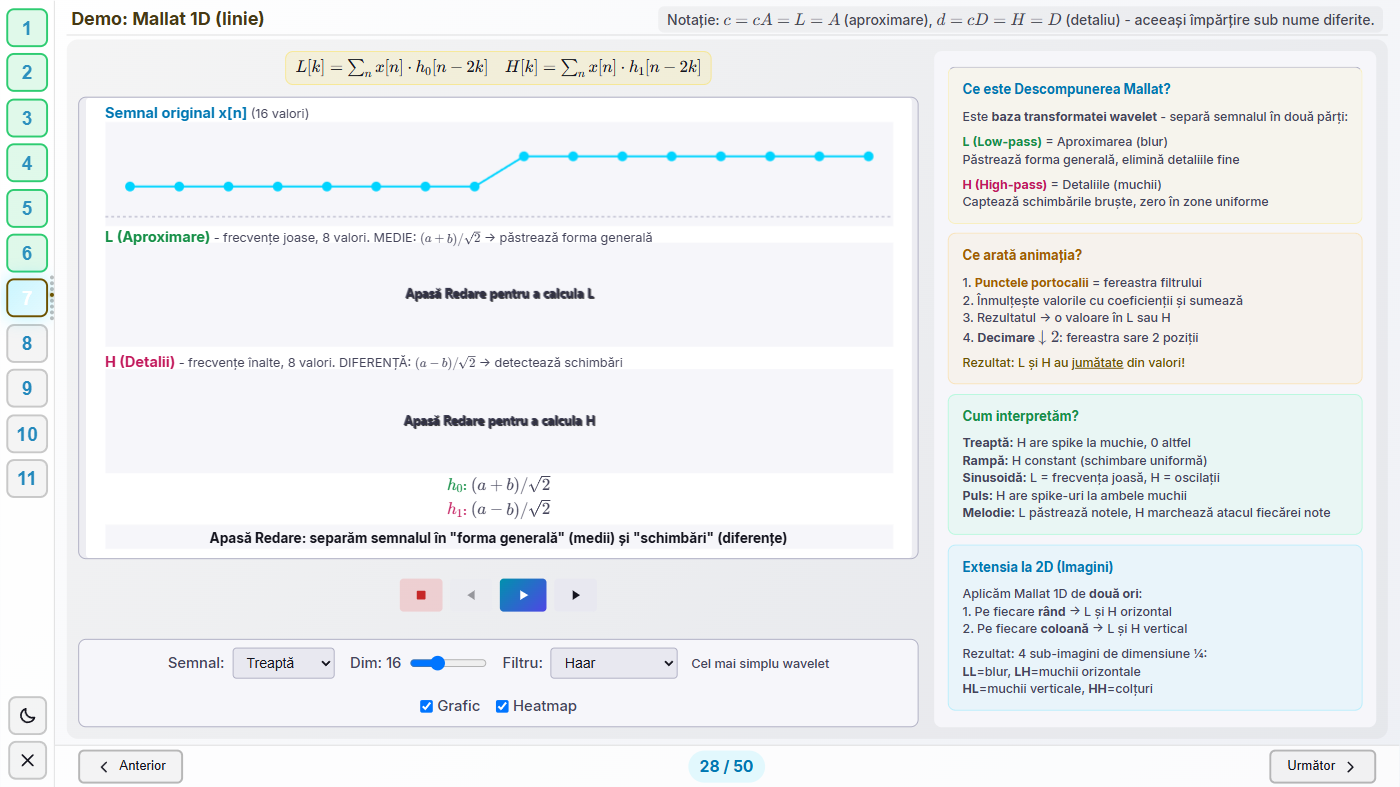
\includegraphics[width=\textwidth]{28-mallat-1d-edu.png}
\caption{Un nivel al algoritmului lui Mallat pas cu pas: fereastra filtrului,
  produsul, suma și decimarea cu doi, pe un semnal treaptă de 16 eșantioane.}
\label{fig:mallat-1d-edu}
\end{figure}

Aplicat recursiv doar pe aproximare, pe patru niveluri
(Figura~\ref{fig:pyramid-recon}, stânga), pasul arată unde se duce energia
unui semnal real: peste 94\% rămâne concentrată în aproximarea cea mai
grosieră, A4. E numărul concret din spatele afirmației că „majoritatea
energiei unei imagini încape într-un număr mic de coeficienți”, premisa pe
care se sprijină toată povestea compresiei din Capitolul~\ref{ch:compresie}.
Un ultim ecran (Figura~\ref{fig:pyramid-recon}, dreapta) arată ce înseamnă
„reconstrucție perfectă” în aritmetică reală: dacă filtrele satisfac
condiția CQF, eroarea rămâne la precizia mașinii de calcul, iar PSNR-ul
raportat reflectă exact acea precizie finită, de aici pornește atât
compresia \emph{lossless}, cât și orice pierdere ulterioară, controlată prin
cuantizare.

\begin{figure}[htbp]
\centering
\begin{subfigure}[t]{0.485\textwidth}
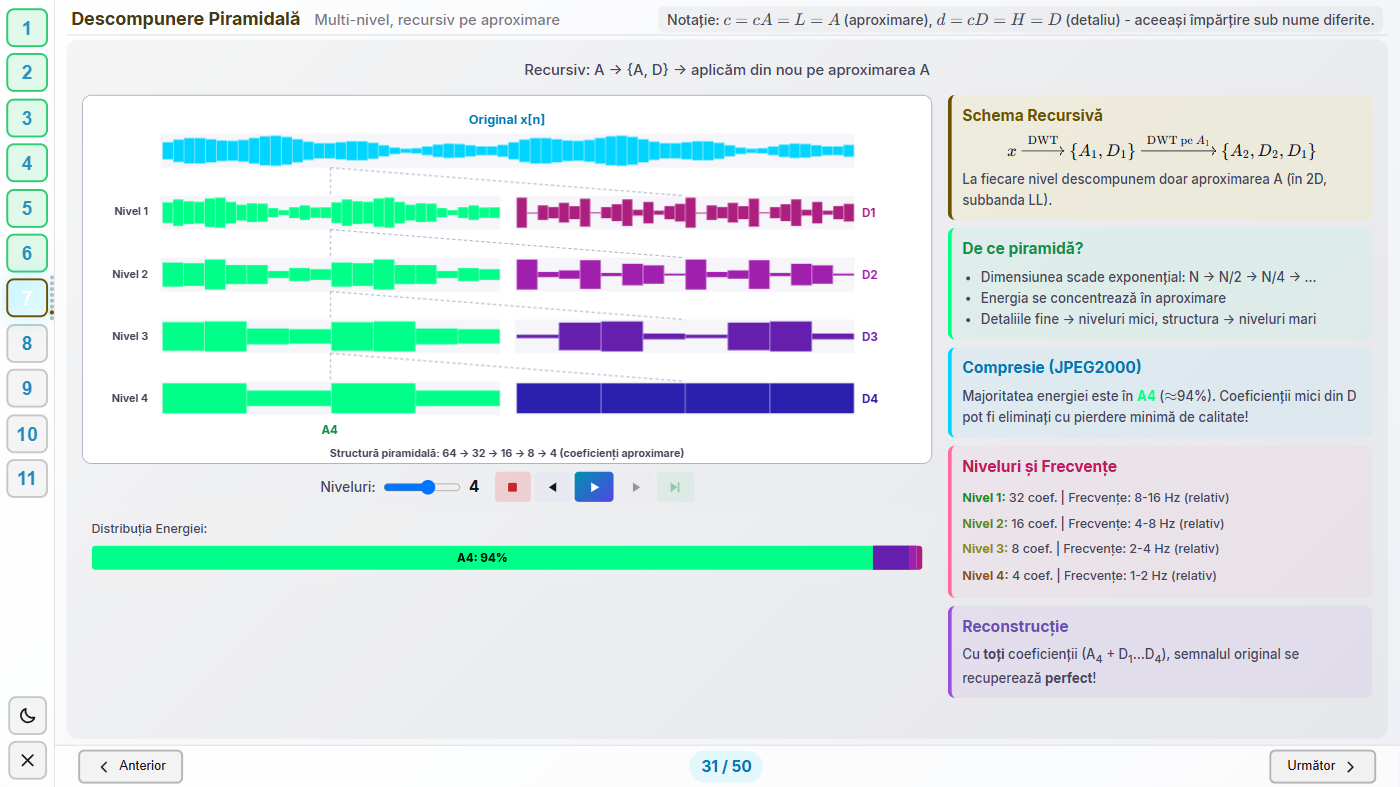
\includegraphics[width=\textwidth]{31-pyramid-decomp.png}
\caption{Patru niveluri recursive: peste 94\% din energie rămâne în A4.}
\end{subfigure}
\hfill
\begin{subfigure}[t]{0.485\textwidth}
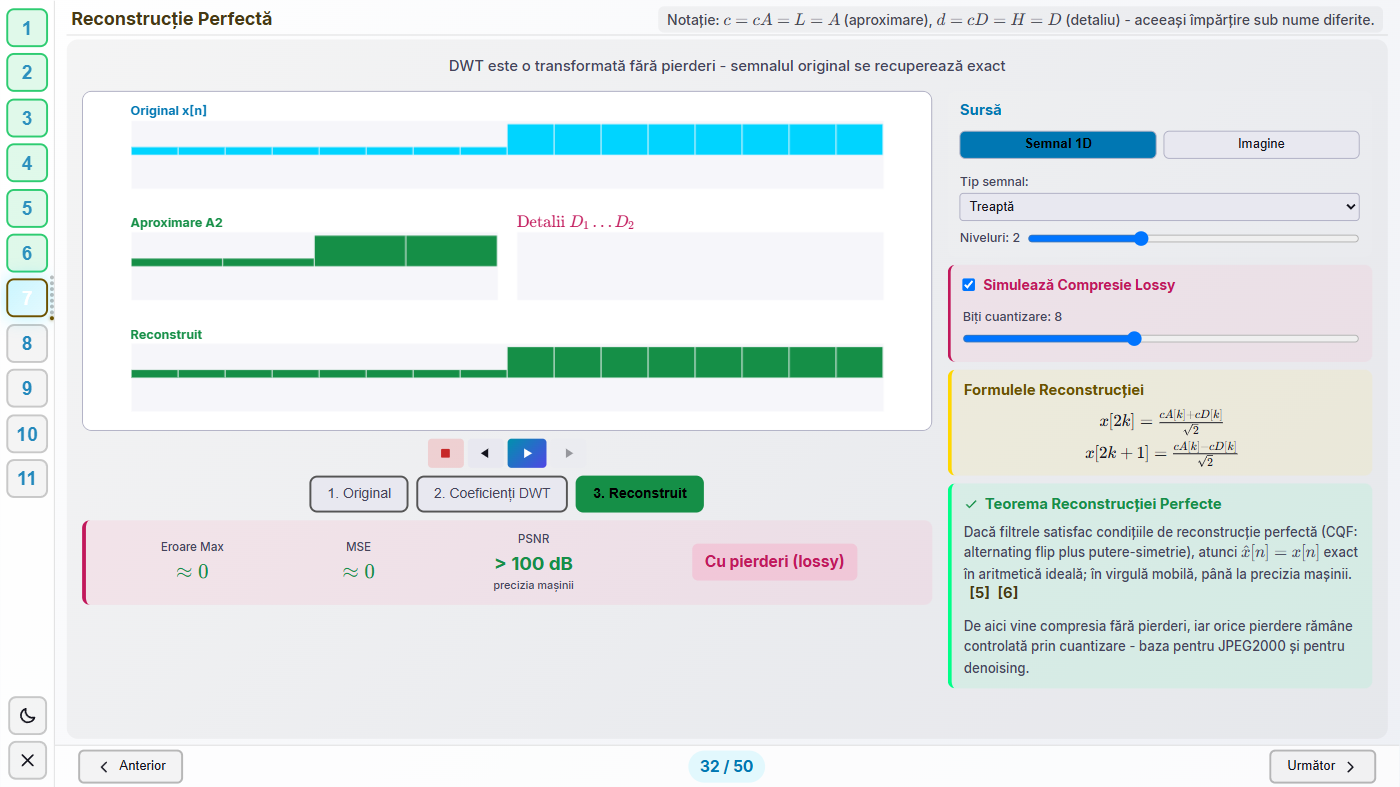
\includegraphics[width=\textwidth]{32-reconstruction.png}
\caption{Reconstrucție perfectă: eroarea rămâne la precizia mașinii, nu la
  zero exact.}
\end{subfigure}
\caption{Multi-nivel (stânga) și reconstrucția care închide bucla (dreapta).}
\label{fig:pyramid-recon}
\end{figure}

Pentru compunerea vizuală a subbenzilor într-un singur mozaic, cum apare pe
mai multe ecrane din tur, fiecare pereche de subbenzi e decupată la
dimensiunea minimă comună înainte de alăturare. PyWavelets poate produce
subbenzi care diferă cu un pixel pe dimensiuni impare de intrare.

\chapter{Compresia imaginilor: JPEG versus JPEG2000}
\label{ch:compresie}

Comprimarea unei imagini se reduce, în ambele standarde, la aceeași idee de
la finalul capitolului trecut: transformă, păstrează coeficienții mari, taie
sau cuantizează grosier restul. JPEG transformă cu DCT pe blocuri mici.
JPEG2000 transformă cu DWT, pe toată imaginea, folosind exact algoritmul lui
Mallat.
Acest capitol arată pipeline-ul JPEG pas cu pas, apoi pune cele două
transformate față în față, la bitrate egal, cu cifre măsurate.

\section{Pipeline-ul JPEG}

Baseline JPEG parcurge șase etape: conversie RGB în YCbCr (separă luminanța
de crominanță), subeșantionare de crominanță (ochiul distinge culoarea mai
slab decât luminozitatea), DCT pe blocuri de $8\times 8$, cuantizare cu
tabelul Annex K scalat după regula IJG, apoi zigzag și codare pe lungimi de
serie. Demo-ul din tur (Figura~\ref{fig:jpeg-pipeline}) rulează toate șase
pe o fotografie reală, nu pe un gradient sintetic, un gradient neted n-are
ce pierde la subeșantionare, deci ar ascunde exact etapa pe care vrea s-o
arate.

\begin{figure}[htbp]
\centering
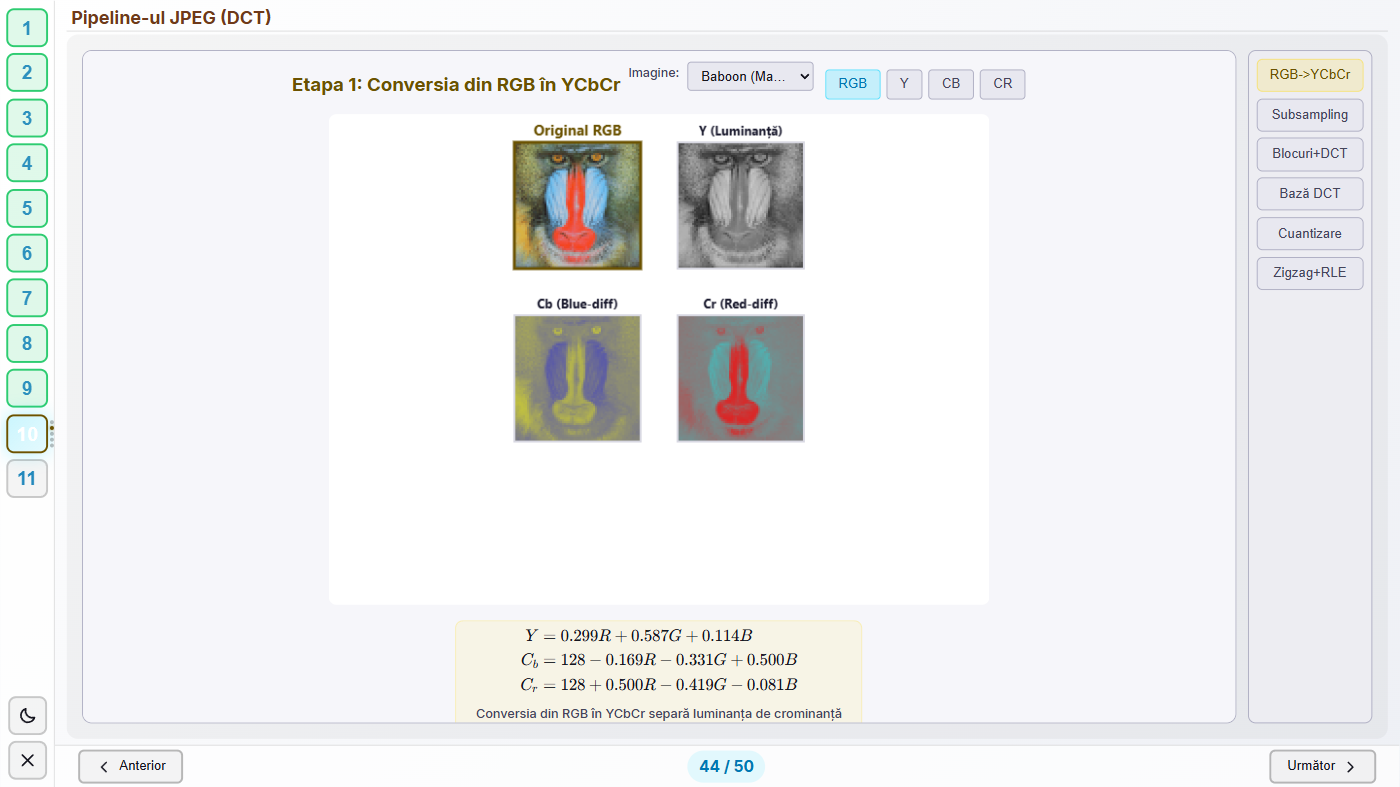
\includegraphics[width=\textwidth]{44-jpeg-pipeline.png}
\caption{Prima etapă a pipeline-ului JPEG pe o fotografie reală: separarea
  Y/Cb/Cr, cu formulele de conversie folosite efectiv de back-end.}
\label{fig:jpeg-pipeline}
\end{figure}

Cele două standarde lasă în urmă tipuri diferite de artefact la compresie
mare. JPEG, cu blocuri independente, lasă blocare: grila de $8\times 8$
devine vizibilă. JPEG2000, cu o transformată globală, lasă
\emph{ringing}~\cite{taubmanmarcellin2002}: oscilații fine în jurul
muchiilor, nu o grilă. JPEG e progresiv doar dacă fișierul e codat explicit
în acel mod din T.81, baseline-ul, cel mai comun pe web, se decodează
secvențial~\cite{itut81}. JPEG2000 capătă scalabilitate progresivă direct
din construcția multi-rezoluție: aceeași descompunere care dă comprimarea dă
și un flux din care poți citi mai întâi o versiune la rezoluție mică, apoi
detaliile~\cite{taubmanmarcellin2002}.

\section{O comparație la bitrate egal}
\label{sec:comparatie}

O primă versiune a acestei comparații compara cele două codecuri la un
parametru de „calitate” egal, calibrat diferit pe fiecare parte, partea DCT
folosea tabelul real Annex K, partea wavelet un prag liniar ad-hoc, fără
nicio legătură cu costul în biți, și scotea un rezultat înșelător, cu JPEG
câștigând la orice calitate testată. Comparația de mai jos egalează
bitrate-ul, nu eticheta de calitate, și măsoară amândouă codecurile cu
același estimator de cost.

\paragraph{Costul în biți.} Fiecare codec e măsurat cu entropia de ordin 0 a
simbolurilor lui cuantizate, înmulțită cu numărul lor,
\[
R = N \cdot H(\mathbf{p}), \qquad H(\mathbf{p}) = -\sum_i p_i \log_2 p_i,
\]
unde $p_i$ e frecvența empirică a simbolului $i$ în histograma
coeficienților cuantizați. Un JPEG sau un JPEG2000 adevărat iese mai mic
decât atât, pentru că folosește o codare entropică reală. Huffman,
aritmetică sau, la JPEG2000, EBCOT cu context, dar cum ambele părți sunt
măsurate cu același estimator, raportul dintre cele două costuri rămâne
comparabil, chiar dacă niciuna dintre cifrele absolute nu e dimensiunea unui
fișier real.

\paragraph{Partea DCT.} Imaginea se taie în blocuri de $8\times 8$ pixeli, iar
fiecare bloc trece prin transformata de cosinus discretă ortonormală,
\[
X_{u,v} = \tfrac14 C_u C_v \sum_{i=0}^{7}\sum_{j=0}^{7} x_{i,j}
  \cos\!\left[\frac{(2i+1)u\pi}{16}\right]
  \cos\!\left[\frac{(2j+1)v\pi}{16}\right], \qquad
C_0 = \tfrac{1}{\sqrt2},\ C_{k>0} = 1,
\]
care scrie blocul ca sumă de $64$ tipare de cosinus, de la cel constant la
cel mai alternant. Urmează cuantizarea cu tabelul de luminanță Annex~K
scalat după regula IJG,
\[
\text{scală} = \begin{cases} 5000/\text{calitate} & \text{calitate} < 50 \\ 200 - 2\cdot\text{calitate} & \text{calitate}\ge 50 \end{cases}, \qquad
Q = \mathrm{clip}\!\left(\left\lfloor \frac{Q_{50}\cdot\text{scală}+50}{100}\right\rfloor,\, 1,\, 255\right).
\]

\paragraph{Partea wavelet primește bugetul de biți al părții DCT.} În loc de
propriul parametru de calitate, partea wavelet caută prin bisecție
geometrică pasul de cuantizare $\Delta$ cel mai fin care încă încape în
bugetul de biți al părții DCT (treizeci de iterații, interval de căutare
$[0.02,\,8192]$, oprire la o precizie relativă de $0.2\%$). Cuantizarea e cu
\emph{zonă moartă}, cu un pas propriu pe fiecare subbandă $b$,
\[
q_b = \mathrm{sign}(c_b)\left\lfloor \frac{|c_b|}{\Delta / g_b}\right\rfloor, \qquad
\hat c_b = \mathrm{sign}(q_b)\left(|q_b|+\tfrac12\right)\frac{\Delta}{g_b},
\]
cu reconstrucția la \emph{mijlocul} intervalului de cuantizare, convenția
standard JPEG2000. Factorul $g_b$ e câștigul de sinteză al subbenzii:
transformata folosită implicit, \txt{bior4.4}, e chiar filtrul 9/7 al
JPEG2000, construit istoric prin schema de \emph{lifting}~\cite{sweldens1998},
iar fiind biortogonală, nu ortonormală, o eroare de un coeficient nu produce
aceeași eroare de reconstrucție în toate subbenzile. Câștigul $g_b$ se
măsoară direct, nu prin formulă: un impuls unitar plasat în centrul
subbenzii, trecut prin transformata inversă singur, iar norma $L_2$ a
rezultatului e $g_b$, exact tehnica JPEG2000 de pași de cuantizare diferiți
pe subbandă~\cite{taubmanmarcellin2002}, aplicată empiric.

\paragraph{Metrici.} PSNR e definiția uzuală,
$\mathrm{PSNR} = 10\log_{10}(255^2/\mathrm{MSE})$. SSIM e implementarea
proprie a formulei lui Wang și colaboratorii,
\[
\mathrm{SSIM}(x,y) = \frac{(2\mu_x\mu_y+C_1)(2\sigma_{xy}+C_2)}{(\mu_x^2+\mu_y^2+C_1)(\sigma_x^2+\sigma_y^2+C_2)}, \qquad
C_1=(0.01L)^2,\ C_2=(0.03L)^2,\ L=255,
\]
pe ferestre $7\times 7$~\cite{wangbovik2004}, verificată numeric față de
\txt{skimage.metrics.structural_similarity}: $0.861644$ (implementare
proprie) față de $0.861132$ (referință) pe imaginea \txt{kodim01} la
calitate 30, diferența venind din tratarea marginilor ferestrei.

\paragraph{Măsurători.} Tabelul~\ref{tab:compare} arată diferența wavelet
minus DCT, la bitrate egal, pentru \txt{bior4.4} pe patru niveluri, pe trei
imagini standard de test.

\begin{table}[htbp]
\centering
\caption{Diferența wavelet minus DCT la bitrate egal (\txt{bior4.4}, 4 niveluri).}
\label{tab:compare}
\begin{tabular}{@{}llrrr@{}}
\toprule
Imagine & Calitate & bpp & $\Delta$PSNR & $\Delta$SSIM \\
\midrule
kodim01 ($768\times 512$) & 10 & 0.512 & $+0.23$~dB & $-0.026$ \\
kodim01 & 20 & 0.865 & $+0.74$~dB & $-0.007$ \\
kodim01 & 30 & 1.132 & $+1.12$~dB & $+0.003$ \\
kodim01 & 50 & 1.522 & $+1.71$~dB & $+0.010$ \\
kodim01 & 75 & 2.159 & $+2.55$~dB & $+0.012$ \\
\txt{peppers_512} & 10 & 0.537 & $-0.33$~dB & $-0.017$ \\
\txt{peppers_512} & 30 & 1.016 & $+0.42$~dB & $-0.011$ \\
\txt{peppers_512} & 50 & 1.319 & $+0.90$~dB & $-0.005$ \\
\txt{baboon_512} & 10 & 0.484 & $+0.12$~dB & $-0.036$ \\
\txt{baboon_512} & 30 & 1.135 & $+0.96$~dB & $+0.006$ \\
\txt{baboon_512} & 50 & 1.567 & $+1.59$~dB & $+0.015$ \\
\bottomrule
\end{tabular}
\end{table}

\emph{Notă}: în ciuda numelui de fișier, \txt{peppers_512}, \txt{baboon_512},
\txt{house_512} și \txt{lake_512} au de fapt $200\times 200$ pixeli.

Demo-ul din tur (Figura~\ref{fig:compare-demo}) rulează exact această
comparație, live, pe imaginea și calitatea alese: la aproximativ 1.01 biți
pe pixel, wavelet câștigă pe PSNR ($+0.93$~dB) și pierde la limită pe SSIM
($-0.001$), cu ambele metrici afișate pe ecran.

\begin{figure}[htbp]
\centering
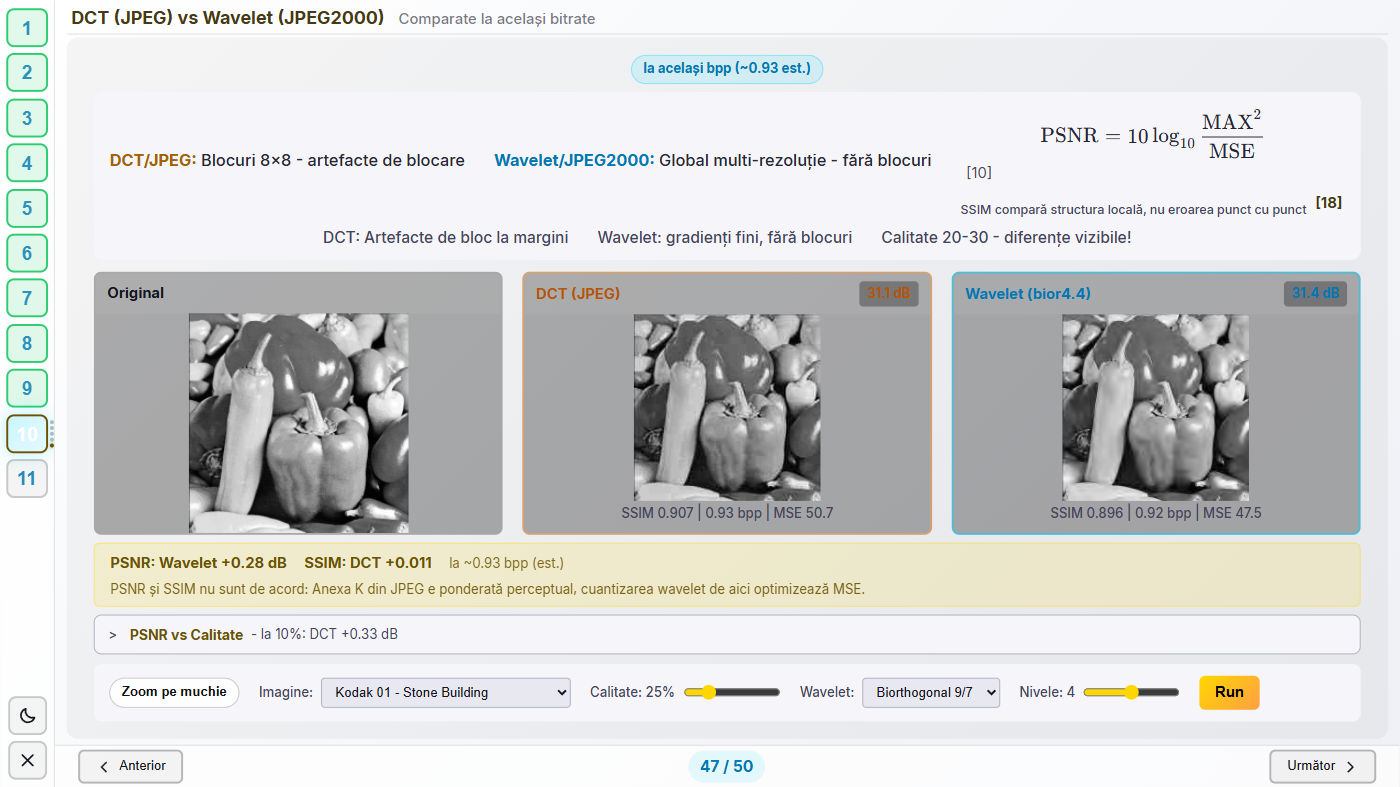
\includegraphics[width=\textwidth]{47-compare-demo.png}
\caption{Comparație la bitrate egal ($\approx 1.01$~bpp): wavelet câștigă pe
  PSNR și pierde la limită pe SSIM, cu ambele metrici afișate pe ecran.}
\label{fig:compare-demo}
\end{figure}

Tabelul spune ceva simplu: wavelet câștigă pe PSNR aproape peste tot, cu
marja crescând odată cu bitrate-ul. SSIM îl favorizează ușor pe JPEG la
bitrate foarte mic, și e un rezultat real, nu o eroare de măsurare, tabelul
Annex K e ponderat perceptual, construit din studii asupra sensibilității la
contrast a ochiului uman, în timp ce cuantizatorul wavelet folosit aici e
optim pe eroare medie pătratică, nu pe percepție. Restul avantajului pe care
JPEG2000 îl are în literatură la bitrate mic vine din codarea entropică cu
context, EBCOT~\cite{taubmanmarcellin2002}, pe care estimatorul de entropie
de ordin 0 folosit aici nu îl modelează: comparația izolează transformata și
cuantizarea, nu codecul complet.

\chapter{Denoising prin prag}
\label{ch:denoising}

Zgomotul produce coeficienți wavelet mici. Semnalul util produce coeficienți
mari. Un prag care taie sau atenuează coeficienții mici, apoi reconstruiește,
elimină zgomotul fără să tocească muchiile, spre deosebire de un filtru
trece-jos clasic, care ar netezi și detaliile utile odată cu zgomotul.

Estimarea zgomotului folosește abaterea mediană absolută a subbenzii celei
mai fine de detaliu,
\[
\hat\sigma = \frac{\mathrm{median}(|d_{\text{fin}}|)}{0.6745},
\]
o alegere robustă: spre deosebire de o deviație standard calculată direct,
nu e trasă în sus de coeficienții mari care poartă semnal.
Pragul universal al lui Donoho și Johnstone,
$\lambda_{\text{universal}} = \hat\sigma\sqrt{2\ln N}$~\cite{donohojohnstone1994},
iar cele două reguli de trunchiere sunt
\[
\eta_{\text{soft}}(x,\lambda) = \mathrm{sign}(x)\max(|x|-\lambda,\,0), \qquad
\eta_{\text{hard}}(x,\lambda) = x\cdot \mathbb{1}(|x|>\lambda).
\]
Soft micșorează continuu coeficienții spre zero, fără discontinuități. Hard
elimină complet ce e sub prag și păstrează exact restul, cu riscul unor
mici artefacte la graniță (Figura~\ref{fig:denoise-theory}).

\begin{figure}[htbp]
\centering
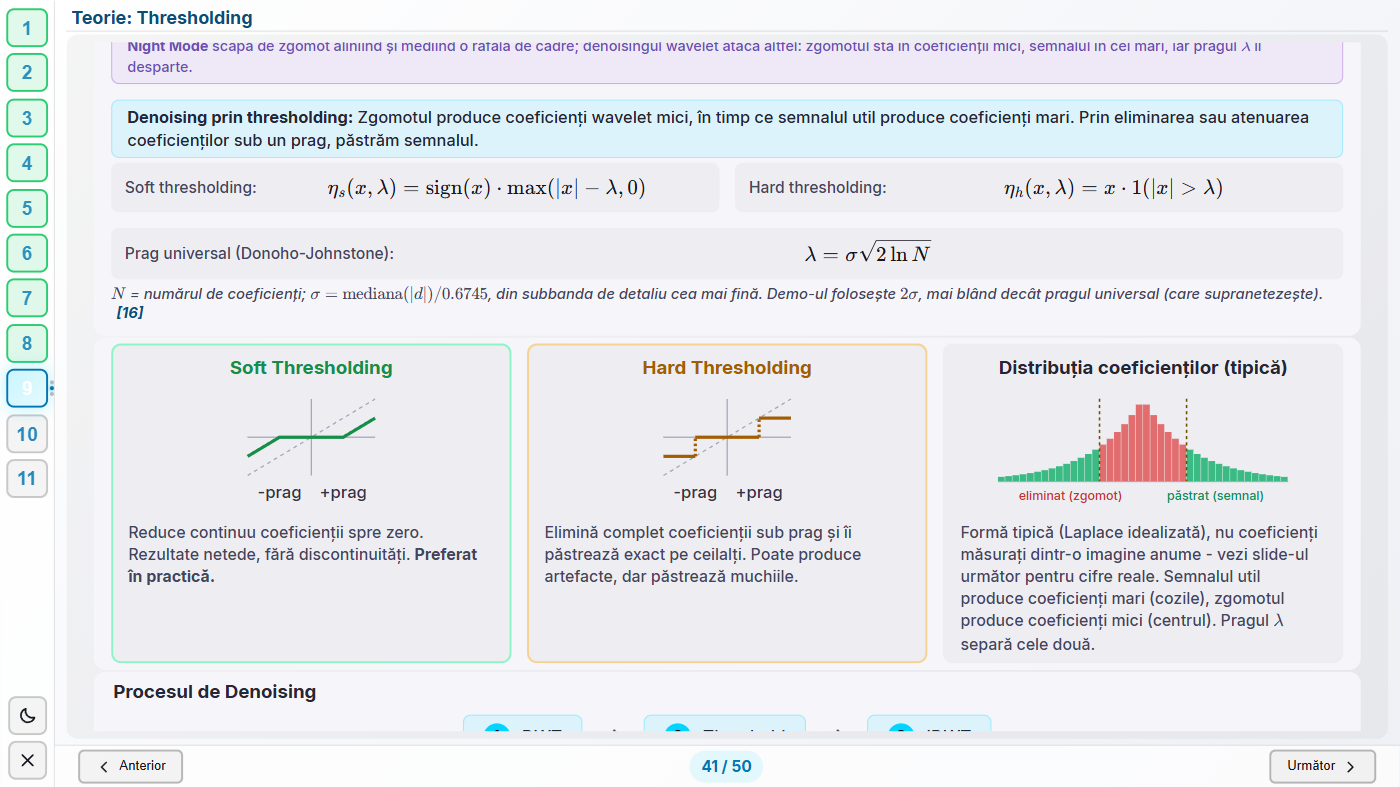
\includegraphics[width=\textwidth]{41-denoise-theory.png}
\caption{Thresholding moale versus dur și distribuția tipică a coeficienților,
  cu pragul universal Donoho-Johnstone alături de pragul $2\hat\sigma$ folosit
  efectiv de demo.}
\label{fig:denoise-theory}
\end{figure}

Pragul folosit efectiv pe imagini e $2\hat\sigma$, mai mic decât pragul
universal din formulă. Abaterea e deliberată și documentată direct în cod. La
$\hat\sigma=15$ și $N=512^2$ (o imagine $512\times 512$), pragul universal
iese în jur de 68, atât de agresiv încât câștigul de raport semnal-zgomot
scade spre $0$~dB: teoria din spatele lui presupune un semnal neted plus
zgomot alb, o ipoteză prea optimistă pentru texturile unei fotografii.
Pragul $2\hat\sigma$ păstrează detaliul și obține în jur de $3$~dB câștig.
Demo-ul de ECG (Capitolul~\ref{ch:ecg}) folosește în schimb chiar pragul
universal, pe un semnal 1D sintetic, unde ipoteza semnal neted plus zgomot
alb se potrivește mult mai bine decât pe o imagine.

Pe o imagine reală (Figura~\ref{fig:denoise-demo}), același proces rulează
cu cifrele la vedere: dincolo de imaginea curățată apare și ce anume s-a
eliminat, amplificat de zece ori, zgomot granular pur, fără nicio structură
a imaginii originale, semn că a rămas doar semnalul.

\begin{figure}[htbp]
\centering
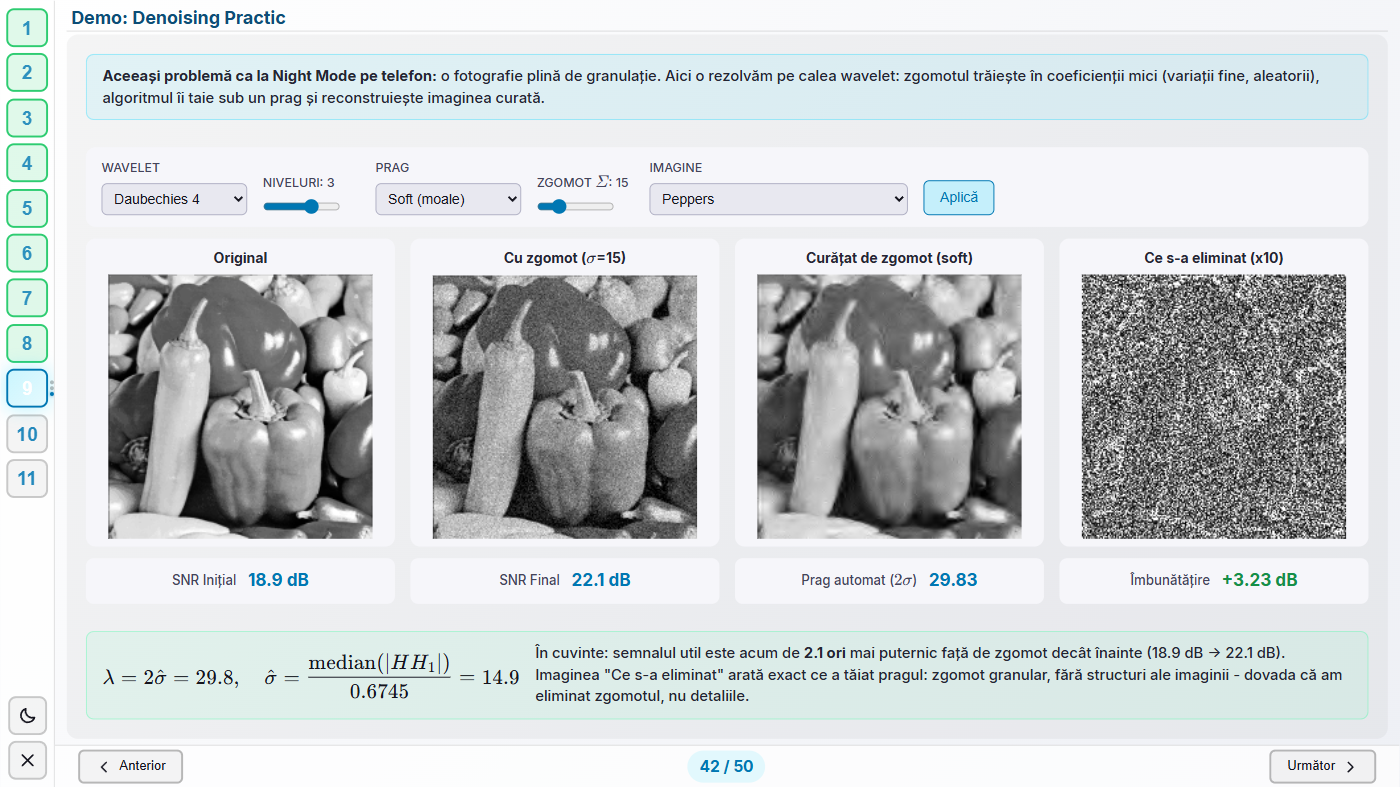
\includegraphics[width=\textwidth]{42-denoise-demo.png}
\caption{Denoising pe o imagine reală: reziduul amplificat $\times 10$ e
  zgomot granular pur, fără nicio structură a imaginii, semn că a rămas
  doar zgomotul.}
\label{fig:denoise-demo}
\end{figure}

\chapter{Aplicație: electrocardiograma}
\label{ch:ecg}

O bătaie de inimă, văzută pe un ECG, e o secvență de unde cu nume proprii: P
marchează depolarizarea atriilor, complexul QRS depolarizarea rapidă a
ventriculilor, vârful ascuțit pe care oricine îl recunoaște dintr-un ECG,
iar T repolarizarea ventriculilor. Diagnosticul clinic se citește din formă,
din durată și din regularitatea intervalelor dintre bătăi, toate trei cer,
mai întâi, să găsești fiecare complex QRS într-un semnal care aproape
niciodată nu e curat.

\section{De ce wavelets, aici}

Un complex QRS e o tranziție bruscă de amplitudine, o \emph{singularitate}
locală, în limbajul procesării de semnal, suprapusă peste zgomot muscular,
interferență electrică și o linie de bază care alunecă lent. Fourier nu
ajută direct: spune ce frecvențe conține semnalul, nu unde anume apare
tranziția. O transformată wavelet, la o scală apropiată de durata tipică a
unui QRS ($\sim$0.08-0.12s), face exact ce trebuie: coeficienții mari
apar acolo unde semnalul se schimbă brusc, restul rămâne mic. E aceeași
proprietate de localizare din Capitolul~\ref{ch:wavelets}, aplicată la un
semnal 1D real.

Martinez, Almeida, Olmos, Rocha și Laguna~\cite{martinez2004} formalizează
ideea într-un algoritm în trei etape: mai întâi detectează complexele QRS,
apoi delimitează fiecare complex, vârfurile undelor individuale, începutul
și sfârșitul lui, și în final localizează undele P și T. Mecanismul de
bază e detecția de singularități prin maxime de modul ale transformatei
wavelet pe mai multe scări: un wavelet construit ca derivata unei funcții de
netezire produce, lângă o tranziție bruscă, o pereche de extreme de semn
opus, iar tranziția însăși cade aproape de trecerea prin zero dintre ele,
teoria generală de detecție a singularităților din
\cite{mallat1989,mallat2008}, aplicată aici la ECG. Pe bazele de date
standard adnotate manual (MIT-BIH Arrhythmia, QT, European ST-T, CSE),
detectorul de QRS obține o sensibilitate de $99.66\%$ și o predictivitate
pozitivă de $99.56\%$, din o mie de bătăi reale, sub patru sunt ratate sau
inventate.

Miza practică e directă: un ceas care anunță fibrilație atrială citește
un semnal de fotopletismografie (PPG) în locul unui ECG de spital. E lumină
reflectată de piele, modulată de pulsul sangvin, din care extrage
neregularitatea intervalelor dintre bătăi, uneori completat cu o singură
derivație de ECG pe electrozi din carcasă~\cite{perez2019}. Fie că sursa e
un ECG de spital pe douăsprezece derivații sau un semnal de încheietură
zgomotos, primul pas practic e același: găsește bătăile.

\section{Demo}

Demo-ul din tur (Figura~\ref{fig:ecg-demo}) construiește un ECG sintetic ca
sumă de gaussiene pentru undele P, Q, R, S, T ale fiecărei bătăi, o
aproximare standard pentru semnale de test, îi adaugă zgomot muscular
reglabil, îl curăță cu o transformată wavelet 1D (Capitolul~\ref{ch:denoising},
cu pragul universal Donoho-Johnstone, potrivit aici pentru că semnalul e
aproape de ipoteza „neted plus zgomot alb”) și detectează vârfurile R ca
maxim pe fereastra fiecărei bătăi. Frecvența cardiacă iese din mediana
intervalelor R-R. În captura din figură, cu zgomotul la $\sigma=0.25$,
toate cele șase bătăi sunt găsite corect, iar raportul semnal-zgomot urcă de
la $-2.9$ la $2.1$~dB.

\begin{figure}[htbp]
\centering
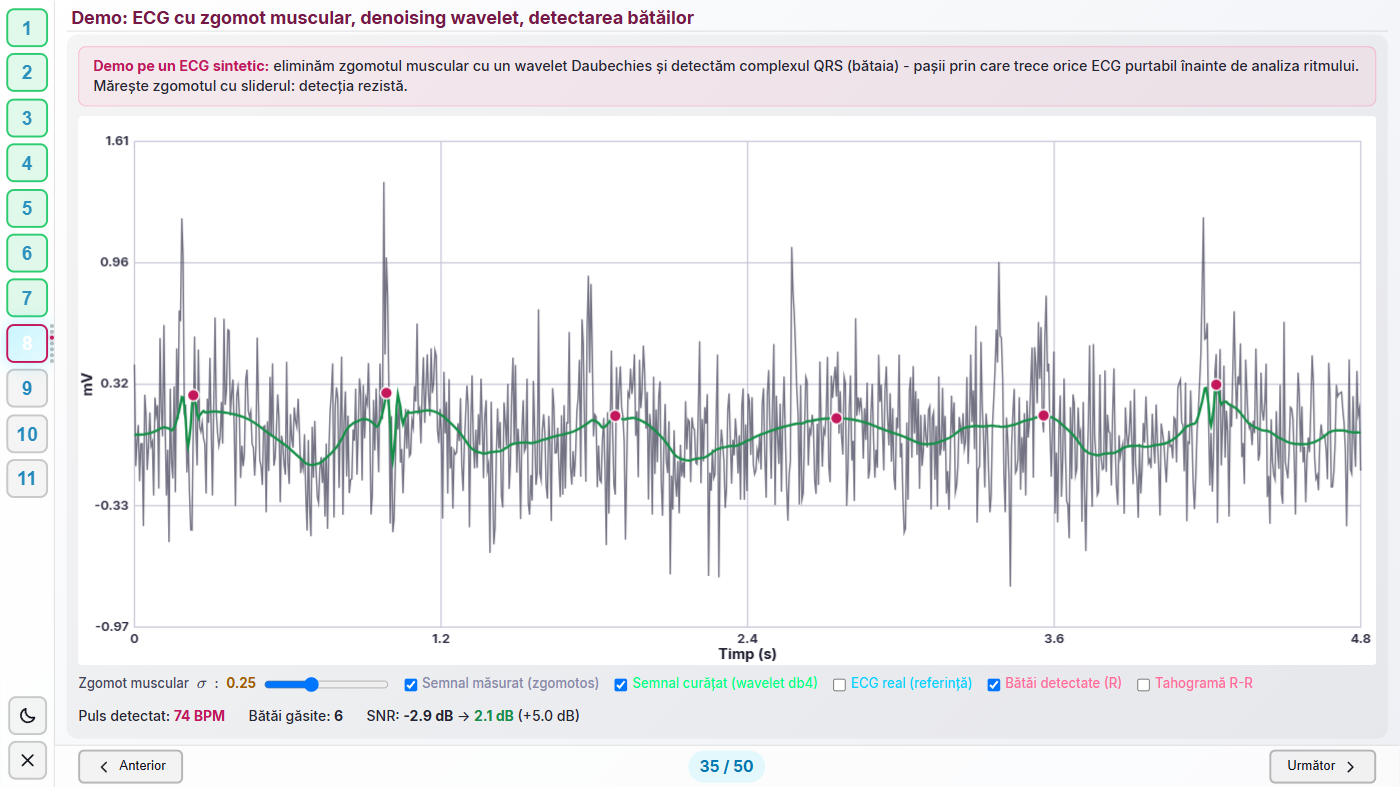
\includegraphics[width=\textwidth]{35-applications-ecg-demo.png}
\caption{ECG sintetic cu zgomot muscular: denoising wavelet și detecția
  celor șase bătăi, SNR de la $-2.9$ la $2.1$~dB.}
\label{fig:ecg-demo}
\end{figure}

\chapter{Aplicație: EEG}
\label{ch:eeg}

Activitatea electrică a creierului, culeasă cu electrozi pe scalp, se
citește pe benzi de frecvență cu semnificație clinică proprie: delta
(0.5-4~Hz, somn profund), theta (4-8~Hz, relaxare adâncă), alfa (8-13~Hz,
ochii închiși, relaxare trează), beta (13-30~Hz, concentrare activă) și
gamma (30-80~Hz, procesare cognitivă complexă). Polisomnografia (studiul
somnului), diagnosticul de epilepsie și interfețele creier-calculator se
bazează, în forme diferite, pe separarea acestor benzi, un ceas care
„estimează” somnul din mișcare și puls nu are acces la niciuna dintre ele.
EEG-ul adevărat rămâne un instrument de laborator sau de clinică.

Demo-ul din tur (Figura~\ref{fig:eeg-demo}) extrage o singură bandă
dintr-un semnal EEG sintetic cu un filtru trece-bandă obișnuit
(Secțiunea~\ref{sec:filtre}), nu cu transformata wavelet discretă folosită
în restul documentului. Motivul e scris direct pe ecran: DWT dublează
frecvența la fiecare nivel, o octavă, dar granițele benzilor clinice nu sunt
spațiate octavă-cu-octavă, delta-theta e aproape un factor de doi,
delta-alfa e deja un factor de $3.25$, așa că niciun set fix de niveluri
DWT nu s-ar alinia cu toate granițele deodată. Un filtru trece-bandă clasic,
cu tăieturi alese liber, nu are această constrângere.

\begin{figure}[htbp]
\centering
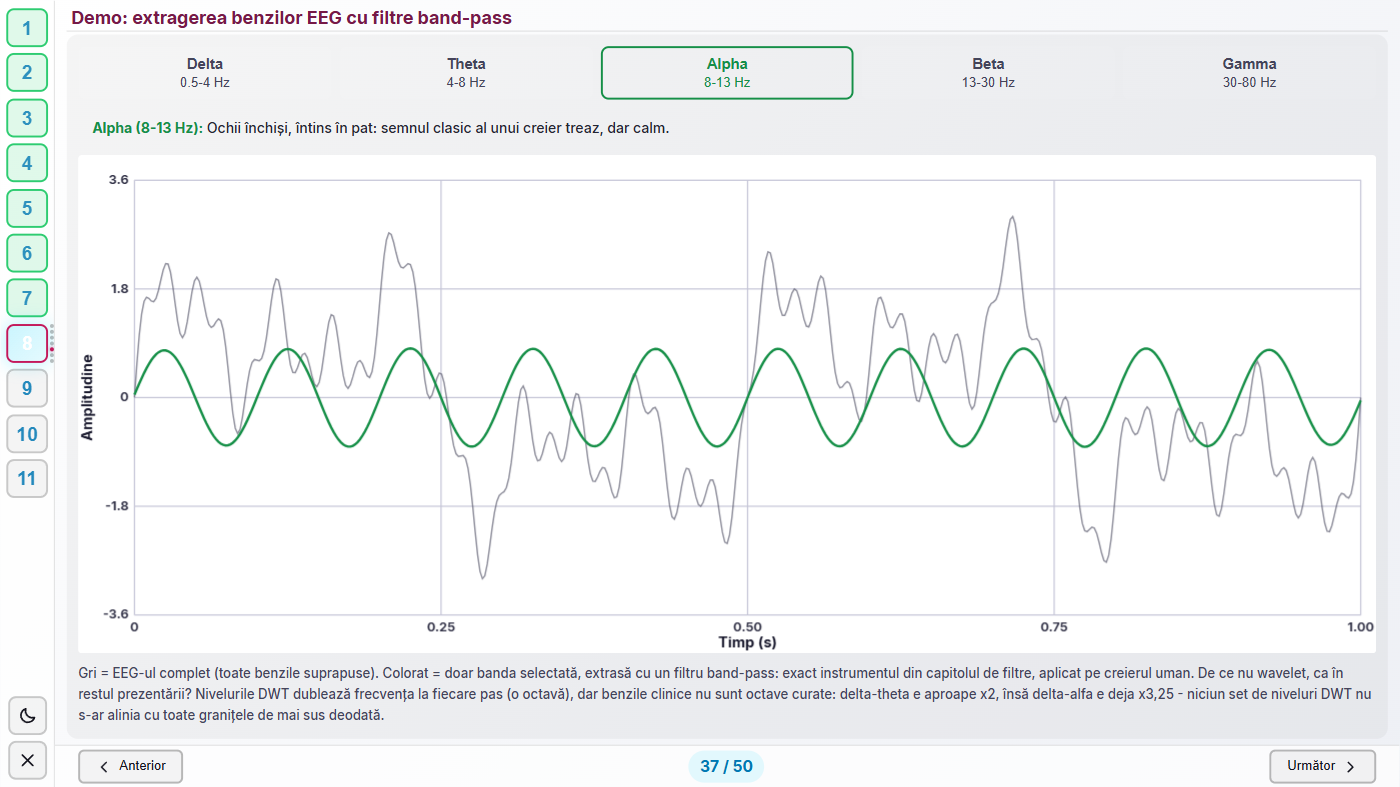
\includegraphics[width=\textwidth]{37-applications-eeg-demo.png}
\caption{Banda alfa (8-13~Hz) extrasă cu un filtru trece-bandă dintr-un EEG
  sintetic. Nota din josul figurii explică de ce nu DWT.}
\label{fig:eeg-demo}
\end{figure}

\chapter{Aplicație: recunoașterea muzicii}
\label{ch:shazam}

Recunoașterea unei piese din câteva secunde de audio, înregistrate cu un
microfon de telefon, peste zgomot de fundal și voci, pare să ceară o
comparație directă cu milioane de piese dintr-o bază de date. Algoritmul
din spatele Shazam~\cite{wang2003} evită exact asta, comparând amprente
scurte și discrete în loc de audio brut.

\section{Cum funcționează amprenta}

Primul pas e o spectrogramă a piesei, exact tipul de reprezentare
timp-frecvență din Capitolul~\ref{ch:wavelets}. Din ea se păstrează doar
vârfurile locale de energie, cele mai puternice puncte din fiecare regiune
de timp-frecvență, alese cu un criteriu de densitate care le distribuie
uniform pe toată durata piesei, cele mai tari câteva din fiecare fereastră,
nu doar cele mai tari câteva sute din tot semnalul.
Rezultatul e o „constelație” de puncte $(t, f)$, suficient de rară ca să
încapă compact, suficient de densă ca să supraviețuiască zgomotului.

Un singur punct din constelație nu spune mare lucru, miile de piese din
bază conțin, fiecare, vârfuri la frecvențe apropiate. Amprenta reală vine
din \emph{perechi}: fiecare punct devine un „punct-ancoră”, legat de câteva
puncte dintr-o „zonă țintă” apropiată în timp și frecvență. Fiecare pereche
(ancoră, țintă) generează un hash format din trei numere, frecvența
ancorei, frecvența țintei și diferența de timp dintre ele,
$(f_1, f_2, \Delta t)$, stocat împreună cu timpul absolut la care apare în
piesă. O piesă de câteva minute produce astfel zeci de mii de hash-uri, nu
un singur „cod” global.

Căutarea unui fragment înregistrat repetă exact procesul, spectrogramă,
constelație, hash-uri, și caută fiecare hash în baza de date. Zgomotul de
fundal adaugă vârfuri false și poate ascunde unele reale, dar tot lasă
destule perechi curate ca zeci de hash-uri să se potrivească exact cu o
singură piesă din bază, iar dacă hash-urile potrivite cad la o diferență de
timp \emph{constantă} față de timpul lor din piesa originală (fragmentul
înregistrat e, de exemplu, exact piesa originală începând din secunda 47),
potrivirea e confirmată statistic, nu doar prin numărul de hash-uri comune.
Pentru că amprenta e locală, fiecare hash descrie doar o mică vecinătate
timp-frecvență, metoda tolerează inclusiv piese suprapuse: hash-urile unei
piese ascultate peste alta rămân, în bună parte, neschimbate, deci ambele
pot fi recunoscute din același fragment.

\section{Demo}

Demo-ul din tur (Figura~\ref{fig:shazam-demo}) arată, mai simplu, punctul de
plecare al ideii: trei acorduri redate pe rând interferează în domeniul
timp, iar semnalul mixt arată vizual de ce identificarea nu se poate face
direct pe formă de undă, notele individuale nu mai sunt separabile cu
ochiul. Textul de pe ecran leagă figura de mecanismul real: vârfurile dintr-o
spectrogramă devin perechi $(f_1, f_2, \Delta t)$ căutate într-o bază de
date, exact procesul descris mai sus.

\begin{figure}[htbp]
\centering
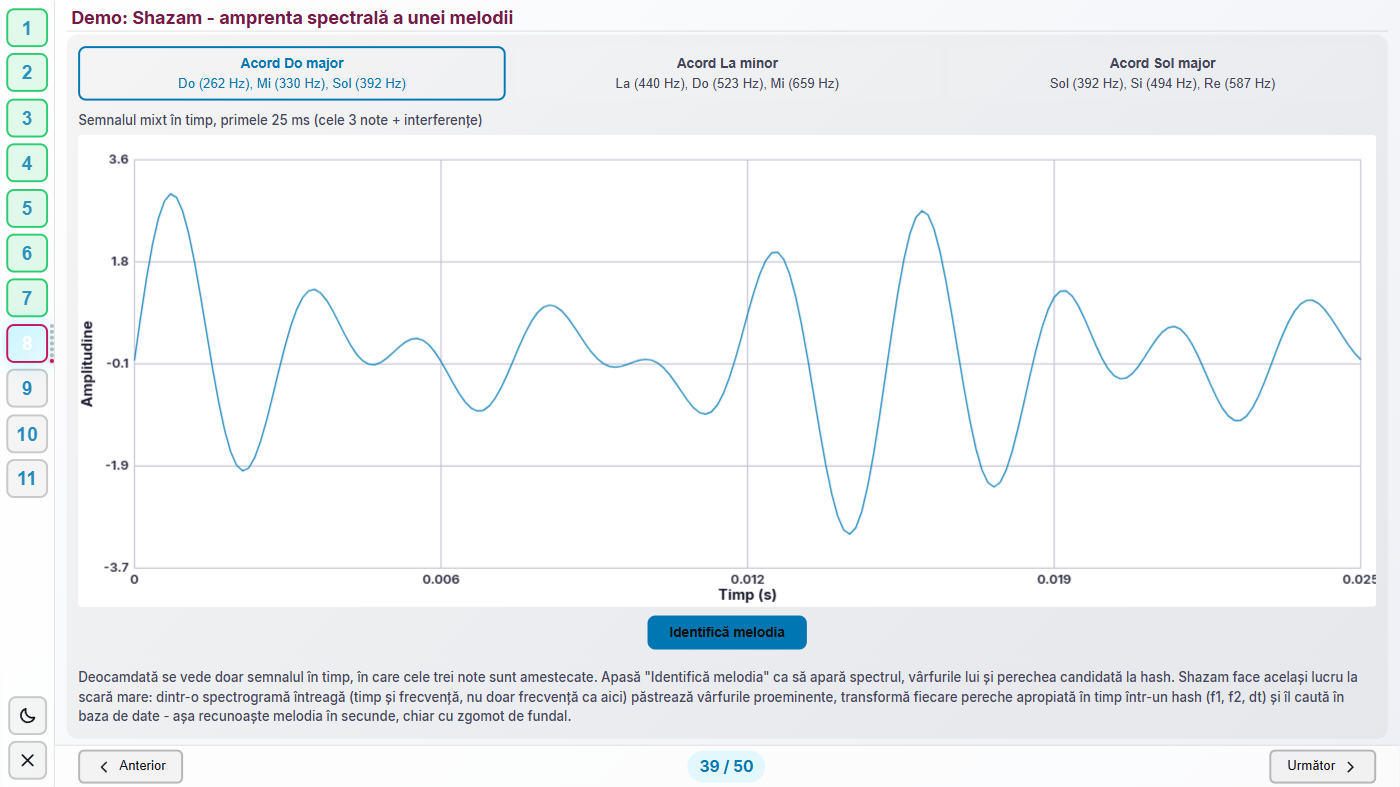
\includegraphics[width=\textwidth]{39-applications-shazam.png}
\caption{Trei acorduri interferând în domeniul timp. Textul explică
  amprentele $(f_1, f_2, \Delta t)$ pe care le caută algoritmul real.}
\label{fig:shazam-demo}
\end{figure}

\chapter{Sinteză: un singur mecanism, multe aplicații}
\label{ch:sinteza}

Dincolo de ECG (Capitolul~\ref{ch:ecg}), EEG (Capitolul~\ref{ch:eeg}) și
recunoașterea muzicii (Capitolul~\ref{ch:shazam}), aceeași transformată apare în
audio (compresie, anularea zgomotului în căști), în securitate cibernetică
(steganografie și \emph{watermarking}, mesaje ascunse în coeficienții HH,
invizibili ochiului), în finanțe (analiza volatilității pe scări de timp),
în seismologie (separarea undelor P și S) și în astronomie (analiza
semnalelor cosmice slabe, îngropate în zgomot).

Privit dintr-o parte, mecanismul e o alegere de dicționar. O bază wavelet e
un dicționar fix, construit dinainte din condiții matematice, în care
semnalele netede pe porțiuni au reprezentări rare, adică puțini coeficienți
mari și restul aproape de zero. Toate capitolele de mai sus exploatează
exact această raritate, fie tăind coeficienții mici ca zgomot, fie
cheltuind biți doar pe cei mari. Întrebarea firească de aici încolo e dacă
dicționarul trebuie ales dinainte sau poate fi învățat din datele înseși,
ceea ce duce la reprezentări rare cu dicționare antrenate, unde baza se
învață din exemplele pe care urmează să le comprime, în locul unei
construcții pornite din condiții teoretice.

Ce leagă toate aplicațiile din acest document e un singur gest, repetat:
descompune semnalul pe scări (aceeași bancă de filtre din
Secțiunea~\ref{sec:mallat}, aplicată recursiv), taie ce nu contează
(zgomot la denoising, biți la compresie, benzi la analiză) și
reconstruiește cu filtrele de sinteză, exact sau controlat de aproape.
Se schimbă doar ce înseamnă „nu contează”: zgomotul muscular la ECG
(Capitolul~\ref{ch:denoising}), biții pe care ochiul nu-i vede la JPEG2000
(Capitolul~\ref{ch:compresie}), tot ce nu e vârf spectral la recunoașterea
muzicii.

\begin{figure}[htbp]
\centering
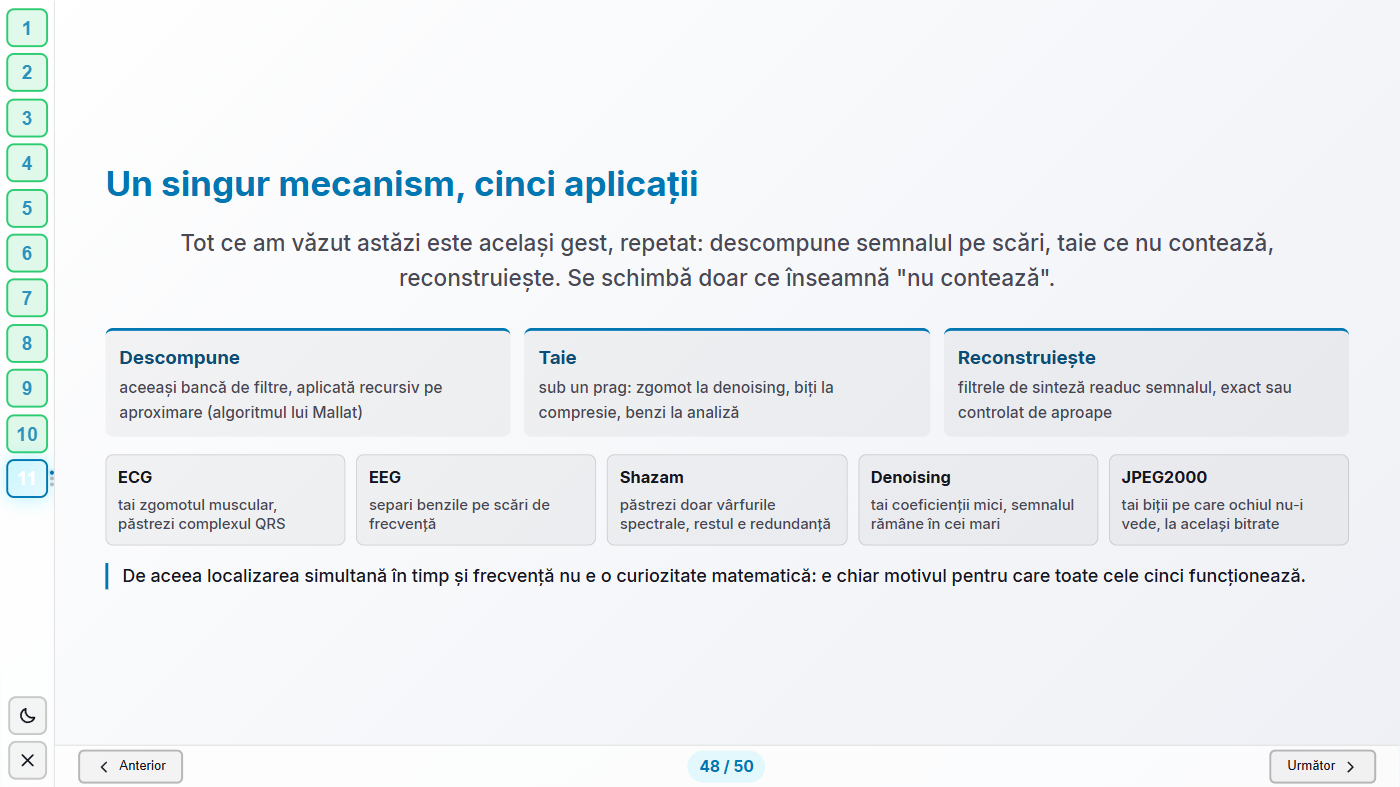
\includegraphics[width=\textwidth]{48-synthesis.png}
\caption{Ecranul de sinteză al turului: descompune / taie / reconstruiește,
  aceleași trei verbe explicând ECG, EEG, recunoașterea muzicii, denoising
  și JPEG2000.}
\label{fig:synthesis}
\end{figure}

Localizarea simultană în timp și frecvență, motivul întregului
Capitolul~\ref{ch:wavelets}, e motivul concret pentru care toate aplicațiile
de mai sus funcționează.

\chapter{Cum e construit, verificat și publicat}
\label{ch:tehnic}

Un ultim capitol, mai scurt, pentru cine vrea să știe și partea de
inginerie din spatele aplicației, nu e conținut de curs, dar explică de ce
demo-urile din capitolele anterioare pot fi luate ca atare.

\section{Pe scurt, arhitectura}

Front-end-ul e React peste Vite. Back-end-ul e FastAPI cu NumPy, SciPy și
PyWavelets. Fiecare ecran e o intrare într-un singur tablou de date, nu un
component separat, iar douăzeci și trei din cele cincizeci montează integral
o componentă de demo interactiv, aceleași componente pe care bara laterală
le poate deschide și individual, în afara turului. Toate desenează pe o
suprafață fixă de $1440\times 810$ pixeli virtuali, scalată proporțional la
fereastra reală, ca un ecran gândit pentru un videoproiector să nu piardă
nimic pe un monitor mai mic.

Calculul e împărțit în două, și distincția merită spusă limpede. Ecranele
care raportează cifre măsurate trimit parametrii către back-end și primesc
înapoi rezultatul unei biblioteci consacrate: filtrele, kernelele pe imagini
reale, denoisingul, comparația la bitrate egal, electrocardiograma și
extragerea benzilor EEG trec toate prin NumPy, SciPy și PyWavelets. Ecranele
care ilustrează un mecanism calculează în browser, cu filtre Haar scrise
direct în JavaScript: descompunerea pas cu pas, banca de filtre, piramida,
reconstrucția, scalograma, cutiile Heisenberg și etapele intermediare ale
pipeline-ului JPEG. Ele arată forma unei idei pe un semnal ales anume, nu o
măsurătoare pe date reale, și de aceea nu poartă cifre pe care textul să se
sprijine.

\section{Verificare automată}
\label{sec:gate}

Corectitudinea vizuală a celor cincizeci de ecrane se verifică prin trei
unelte separate, fiecare acoperind o clasă diferită de defect, în loc de o
singură trecere manuală.

Prima parcurge tot turul într-un browser real și verifică opt clase de
problemă pe fiecare ecran (Tabelul~\ref{tab:gate}), plus erorile de consolă
JavaScript. Conform ultimei rulări complete, verificarea e curată pe toate
cele cincizeci de ecrane, la două rezoluții diferite.

\begin{table}[htbp]
\centering
\caption{Cele opt clase de defect verificate automat pe fiecare ecran.}
\label{tab:gate}
\small
\begin{tabular}{@{}lp{10.3cm}@{}}
\toprule
Clasă & Ce detectează \\
\midrule
\txt{pageScroll} & Suprafața de design scrolează, conținutul depășește $1440\times 810$. \\
\txt{outOfFrame} & Un element vizibil (buton, input, imagine, canvas, text) iese din
  viewport, cu toleranță de 2 pixeli. \\
\txt{innerScroll} & Un element are conținut tăiat sau scrolabil intern
  (\txt{scrollHeight} peste \txt{clientHeight}). \\
\txt{overlaps} & Două elemente vizibile fără relație de descendență se
  suprapun cu cel puțin 6 pixeli pe ambele axe. \\
\txt{occludedControls} & Un control al cărui centru, testat la trei
  înălțimi, indică sub cursor un element diferit, prinde acoperirea de
  către un element exclus din \txt{overlaps}, de exemplu un \txt{canvas}. \\
\txt{smallMath} & O formulă KaTeX randată sub pragul de lizibilitate (14px
  inline, 18px afișată, în pixeli de design). \\
\txt{rawTokens} & Un token \texttt{\$...\$} sau \txt{[cite:...]} ajuns pe ecran ca
  text brut. \\
\txt{duplicateTitles} & Un ecran de tip \txt{embed} își afișează propriul
  titlu, deasupra titlului din metadata turului. \\
\bottomrule
\end{tabular}
\end{table}

A doua unealtă merge mai departe decât o simplă citire: apasă efectiv
fiecare buton, mișcă fiecare cursor, comută fiecare selector și bifează
fiecare căsuță de pe fiecare ecran, cu o captură înainte și una după fiecare
acțiune (Figura~\ref{fig:kernels-edu-interaction}). Măsoară dacă vreun
element s-a deplasat neașteptat pe ecran, verifică geometric dacă imaginile
și canvas-urile rămân în interiorul cutiei lor și colectează orice eroare
nouă de consolă. Ultima rulare completă a apăsat sau tras 911 controale, pe
toate cele cincizeci de ecrane, fără niciunul lipsit de un nume accesibil și
fără nicio eroare.

\begin{figure}[htbp]
\centering
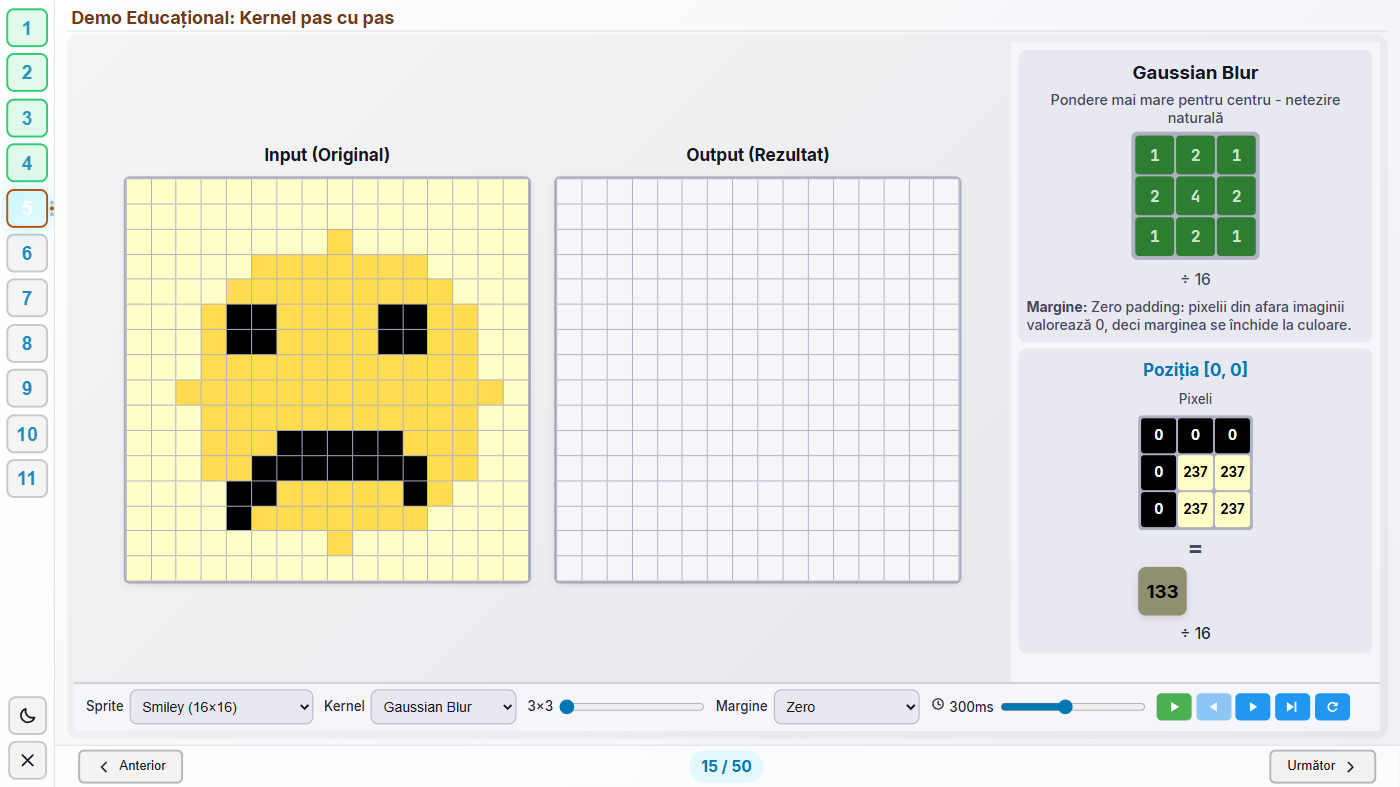
\includegraphics[width=\textwidth]{15-kernels-edu.png}
\caption{Un ecran tipic pentru trecerea de interacțiune: selector de sprite,
  selector de kernel, cursor de dimensiune, selector de margine, cursor de
  viteză și cinci butoane de transport, fiecare apăsat sau tras automat, cu
  o captură înainte și una după.}
\label{fig:kernels-edu-interaction}
\end{figure}

A treia unealtă scanează codul sursă, nu ecranul: caută orice caracter
Unicode folosit în locul unei formule LaTeX sau al unei iconițe proprii de
interfață, pe principiul că matematica se randează mereu prin LaTeX, iar
orice iconiță e un desen propriu, nu un caracter de font care arată diferit
de la un sistem la altul. E curată pe tot front-end-ul.

Niciuna dintre cele trei unelte nu vede ce se desenează în interiorul unui
element de tip canvas, și acolo trăiesc majoritatea graficelor din tur:
spectre, răspunsuri de filtru, forme de wavelet, scalograme. O suprapunere
între o etichetă și o linie de grilă, acolo, nu apare în niciun raport
automat. Compensarea e directă: citirea capturilor de ecran salvate de
aceste unelte, ecran cu ecran, exact așa au fost alese și cele douăzeci și
două de figuri din acest document.

\section{Rulare locală}

Back-end-ul pornește din \txt{backend/}, după instalarea dependențelor
(FastAPI, Uvicorn, NumPy, SciPy, Pillow, PyWavelets, Pydantic). Front-end-ul
pornește din \txt{frontend/}, după \texttt{npm install}. Serverul de dezvoltare
Vite redirecționează automat orice cerere către \txt{/api} spre back-end,
așa că front-end-ul n-are niciun URL scris în cod, nici măcar în dezvoltare.
Fiecare ecran al turului se deschide direct, cu propriul \emph{deep link}.

\section{Publicarea pe server}

Aplicația rulează dintr-o singură imagine Docker, construită în doi pași:
front-end-ul se compilează întâi, apoi rezultatul e copiat peste back-end,
care ajunge astfel să servească, pe același port, și pagina, și API-ul.
Local, imaginea se construiește și pornește cu o singură comandă
\texttt{docker compose}.

Publicarea la \url{https://ale0204.student-dev.ro/dsp/} nu construiește nimic
pe mașina de acasă: sursa proiectului se împachetează și se trimite pe
server, imaginea se construiește direct acolo, deci mașina de acasă n-are
nevoie de Docker instalat sau pornit, doar trimite codul, iar la final
containerul pornește în spatele reverse proxy-ului serverului, care termină
conexiunea securizată și trimite mai departe cererile către aplicație.
Containerul nu publică niciun port propriu.

Fișierele care descriu un server anume, rețeaua în care intră containerul,
contul și directorul de pe gazdă, stau în afara depozitului public, pentru
că depind de gazdă, nu de aplicație. Depozitul rămâne astfel rulabil de
oricine, oriunde, fără nicio adresă scrisă în cod.

% ============================================================
\chapter*{Bibliografie}
\addcontentsline{toc}{chapter}{Bibliografie}

Ordinea de mai jos e cea din registrul sursă al aplicației
(\txt{frontend/src/components/shared/sources.js}), ordinea primei apariții a
fiecărei surse în tur, astfel încât numărul \txt{[n]} din orice figură a
acestui document coincide cu numărul citat de aplicație.

\begin{thebibliography}{99}

\bibitem{dci2024} Digital Cinema Initiatives. \emph{Digital Cinema System
  Specification}, v1.4.4, secțiunea 4.2. DCI, LLC, 2024.
  \url{https://documents.dcimovies.com/DCSS/}

\bibitem{wang2003} A. L. Wang. \emph{An industrial-strength audio search
  algorithm}. Proc. ISMIR, 2003.
  \url{https://www.ee.columbia.edu/~dpwe/papers/Wang03-shazam.pdf}

\bibitem{lyons2011} R. G. Lyons. \emph{Understanding Digital Signal
  Processing}, ediția a 3-a. Prentice Hall, 2011.

\bibitem{strangnguyen1996} G. Strang, T. Nguyen. \emph{Wavelets and Filter
  Banks}. Wellesley-Cambridge Press, 1996.

\bibitem{estebangaland1977} D. Esteban, C. Galand. \emph{Application of
  quadrature mirror filters to split band voice coding schemes}. Proc. IEEE
  ICASSP, 1977. \url{https://doi.org/10.1109/ICASSP.1977.1170341}

\bibitem{smithbarnwell1984} M. J. T. Smith, T. P. Barnwell III. \emph{A
  procedure for designing exact reconstruction filter banks for
  tree-structured subband coders}. Proc. IEEE ICASSP, 1984.
  \url{https://doi.org/10.1109/ICASSP.1984.1172486}

\bibitem{shannon1949} C. E. Shannon. \emph{Communication in the presence of
  noise}. Proc. IRE 37(1), 10-21, 1949.
  \url{https://doi.org/10.1109/JRPROC.1949.232969}

\bibitem{daubechies1992} I. Daubechies. \emph{Ten Lectures on Wavelets}.
  SIAM, 1992. \url{https://doi.org/10.1137/1.9781611970104}

\bibitem{daubechies1988} I. Daubechies. \emph{Orthonormal bases of compactly
  supported wavelets}. Comm. Pure Appl. Math. 41(7), 1988.
  \url{https://doi.org/10.1002/cpa.3160410705}

\bibitem{taubmanmarcellin2002} D. S. Taubman, M. W. Marcellin. \emph{JPEG2000:
  Image Compression Fundamentals, Standards and Practice}. Kluwer Academic,
  2002.

\bibitem{sweldens1998} W. Sweldens. \emph{The lifting scheme: A construction
  of second generation wavelets}. SIAM J. Math. Anal. 29(2), 1998.
  \url{https://doi.org/10.1137/S0036141095289051}

\bibitem{mallat2008} S. Mallat. \emph{A Wavelet Tour of Signal Processing:
  The Sparse Way}, ediția a 3-a. Academic Press, 2008.
  \url{https://www.sciencedirect.com/book/9780123743701/a-wavelet-tour-of-signal-processing}

\bibitem{mallat1989} S. Mallat. \emph{A theory for multiresolution signal
  decomposition: the wavelet representation}. IEEE Trans. Pattern Anal.
  Mach. Intell. 11(7), 674-693, 1989. \url{https://doi.org/10.1109/34.192463}

\bibitem{perez2019} M. V. Perez et al. (Apple Heart Study). \emph{Large-scale
  assessment of a smartwatch to identify atrial fibrillation}. N. Engl. J.
  Med. 381(20), 1909-1917, 2019. \url{https://doi.org/10.1056/NEJMoa1901183}

\bibitem{martinez2004} J. P. Martínez, R. Almeida, S. Olmos, A. P. Rocha, P.
  Laguna. \emph{A wavelet-based ECG delineator: evaluation on standard
  databases}. IEEE Trans. Biomed. Eng. 51(4), 570-581, 2004.
  \url{https://doi.org/10.1109/TBME.2003.821031}

\bibitem{donohojohnstone1994} D. L. Donoho, I. M. Johnstone. \emph{Ideal
  spatial adaptation by wavelet shrinkage}. Biometrika 81(3), 425-455, 1994.
  \url{https://doi.org/10.1093/biomet/81.3.425}

\bibitem{itut81} ITU-T. \emph{Rec. T.81: Digital compression and coding of
  continuous-tone still images}. ITU-T / ISO-IEC 10918-1, 1992.
  \url{https://www.w3.org/Graphics/JPEG/itu-t81.pdf}

\bibitem{wangbovik2004} Z. Wang, A. C. Bovik, H. R. Sheikh, E. P. Simoncelli.
  \emph{Image quality assessment: from error visibility to structural
  similarity}. IEEE Trans. Image Process. 13(4), 600-612, 2004.
  \url{https://doi.org/10.1109/TIP.2003.819861}

\bibitem{oppenheimschafer2010} A. V. Oppenheim, R. W. Schafer.
  \emph{Discrete-Time Signal Processing}, ediția a 3-a. Prentice Hall, 2010.

\end{thebibliography}


\end{document}
